% !TEX root = ../TAMU_Thesis_Main.tex

%%%%%%%%%%%%%%%%%%%%%%%%%%%%%%%%%%%%%%%%%%%%%%%%%%%%%%%%%%%%%%%%%%%%%%%
%%%                           SECTION IV
%%%%%%%%%%%%%%%%%%%%%%%%%%%%%%%%%%%%%%%%%%%%%%%%%%%%%%%%%%%%%%%%%%%%%%


\chapter{Towards the assessment of submesoscale processes in regionally refined MPAS-O simulations of the Gulf of Mexico}

\section{Abstract}
Submesoscale oceanic processes (submesoscales) are posited to be important for the global climate system. However, computational constraints limit the global ocean component of the U.S. Department of Energy's Exascale Earth System Model, the Model for Prediction Across Scales-Ocean (MPAS-O), from globally resolving submesoscales in fully coupled simulations for the foreseeable future. This work presents the development of an unprecedented 2.8 km resolution regionally refined mesh in the Gulf of Mexico (GoM), which is intended to assess the representation of coastal submesoscales and Mississippi/Atchafalaya (M/A) River plume over the Texas-Louisiana (TXLA) shelf and the broader GoM. We document the horizontal and vertical mesh design processes, improvements made to river spreading, and tuning of key subgrid-scale parameterizations. Model results are compared with the validated TXLA shelf model. We ran simulations using low (GoM3r1) and medium (GoM3r2) vertical resolution meshes for two years (2000-2001). A key result is that MPAS-O experiences stability issues at comparable vertical resolution to the TXLA model. While both simulations permit submesoscale seasonal variability in the broader GoM, they poorly represent submesoscales over the TXLA shelf and do not produce an eddy field during summer. GoM3r1 does not the represent surface structure of the M/A plume due to the coarse resolution. GoM3r2 demonstrates some qualitative agreement with the TXLA model, with salty biases near Atchafalaya Bay and fresher biases over the southern TX coast. We anticipate improved performance upon resolution of stability issues and further improvement of river spreading.

\section{Introduction}
Coastal regions are under increasing environmental stressors due to anthropogenic climate change and human activities. For example, rising sea levels, increasing storm intensity, and marine pollution have profound impacts on the well-being of society and will cause billions of dollars in economic damages in coming decades \citep{RN23}. Consequently, the U.S. Department of Energy (DOE) has directed significant effort towards developing the Energy Exascale Earth System Model (E3SM), allowing us to improve our understanding of Earth's climate \citep{golaz2022doe}. E3SM component meshes possess multiresolution capabilities \citep{ringler2008multiresolution}, which allow for regional refinement over a prescribed area. An advantage of multiresolution capabilities relative to other ESMs that use structured grids \citep[e.g., the Community Earth System Model, ][]{danabasoglu2020community} is that a regionally refined mesh can represent similar dynamics as a globally uniform high resolution configuration in the region of interest but with 10-20\% of the computational cost \citep{tang2023fully}. 

One of the most pressing challenges facing E3SM development is parameterizing and representing submesoscale ocean processes (submesoscales) within the Model for Prediction Across Scales-Ocean \citep[MPAS-O,][]{ringler2013multi}. The defining dynamical characteristic of submesoscales is their $\mathcal{O}$(1) Rossby number, which results in large vertical motions relative to their mesoscale counterparts. Several reviews \citep{McWilliams_2016,mcwilliams2019survey,taylor2023submesoscale} highlight various mechanisms by which submesoscales can influence regional and global climates, although new processes are still being discovered. 

For example, over the Texas-Louisiana (TXLA) continental shelf in the northern Gulf of Mexico (nGoM), summertime stratification of nutrient-rich brackish water from the Mississippi/Atchafalaya (M/A) river plume and saltier ocean water contributes to the formation of bottom hypoxia, annually forming one of largest dead zones in the world \citep{bianchi2010science, ruiz2021small}. A diurnal land-sea breeze in near-resonance with the regional inertial period interacts with density fronts associated with the plume’s submesoscale eddy field \citep{Hetland_2017, Kobashi_2020}. The resulting convergence and divergence at the fronts leads to a slantwise circulation where surface water is subducted along isopycnals and bottom water is ventilated \citep{qu2022rapid}. The slantwise vertical circulation was discovered in triple-nested, nonhydrostatic TXLA model simulations configured as part of the Coastal and Regional Ocean COmmunity Model (\url{https://www.croco-ocean.org/}), which is based on the Regional Ocean Modeling Systems \citep[ROMS, ]{shchepetkin2005regional}. While the larger-scale biogeochemical impacts of this process remains unclear, it is one example of an unaccounted process in E3SM. 

E3SM’s utility for forecasting changes to coastal regions is severely constrained by grid resolution, a dominant parameter controlling earth system model error and bias. However, increasing grid resolution is not guaranteed to increase model fidelity because larger-scale models may lack appropriate, grid-scale aware parameterizations, or they may use parameterizations that are ill-posed for modeling coastal processes. Furthermore, even with its regional mesh refinement capabilities, global MPAS-O simulations are unlikely to achieve the $\mathcal{O}$(1 km) horizontal resolution required to resolve many coastal ocean processes in the next decade. \cite{hoch2020mpas} assessed MPAS-O fidelity for two regionally refined meshes with 8 km resolution over the coastal United States (CUSP8) and North Atlantic (NA8). However, these simulations were run in ``stand alone'', which used constant data-derived, atmospheric forcing and were uncoupled from the E3SM atmosphere, sea ice, river transport, and land models. The current high resolution mesh used in fully-coupled simulations (RRS18to6) features a minimum resolution of 6 km near the poles that is relaxed to 18 km near the equator \citep[see Fig. 2 of ][]{caldwell2019doe}, making it insufficient to resolve the first baroclinic deformation radius in many coastal regions. 

Thus, there is a pressing need to assess MPAS-O's representation of submesoscale coastal processes so the model's strengths and limitations can be identified as E3SM simulations push towards higher resolutions. The primary objective of this work is to report preliminary efforts to produce regionally refined simulations of the nGoM using MPAS-O. We present the development of a submesoscale permitting, regionally refined mesh that has a 2.8 km resolution within the GoM and a courser resolution elsewhere (Fig. \ref{fig:mesh_overview} c). The results of this study can be used to help guide the development of future submesoscale-permitting coastal E3SM simulations. Our case study approach is motivated by several factors.

\begin{figure}[t!]
\centerline{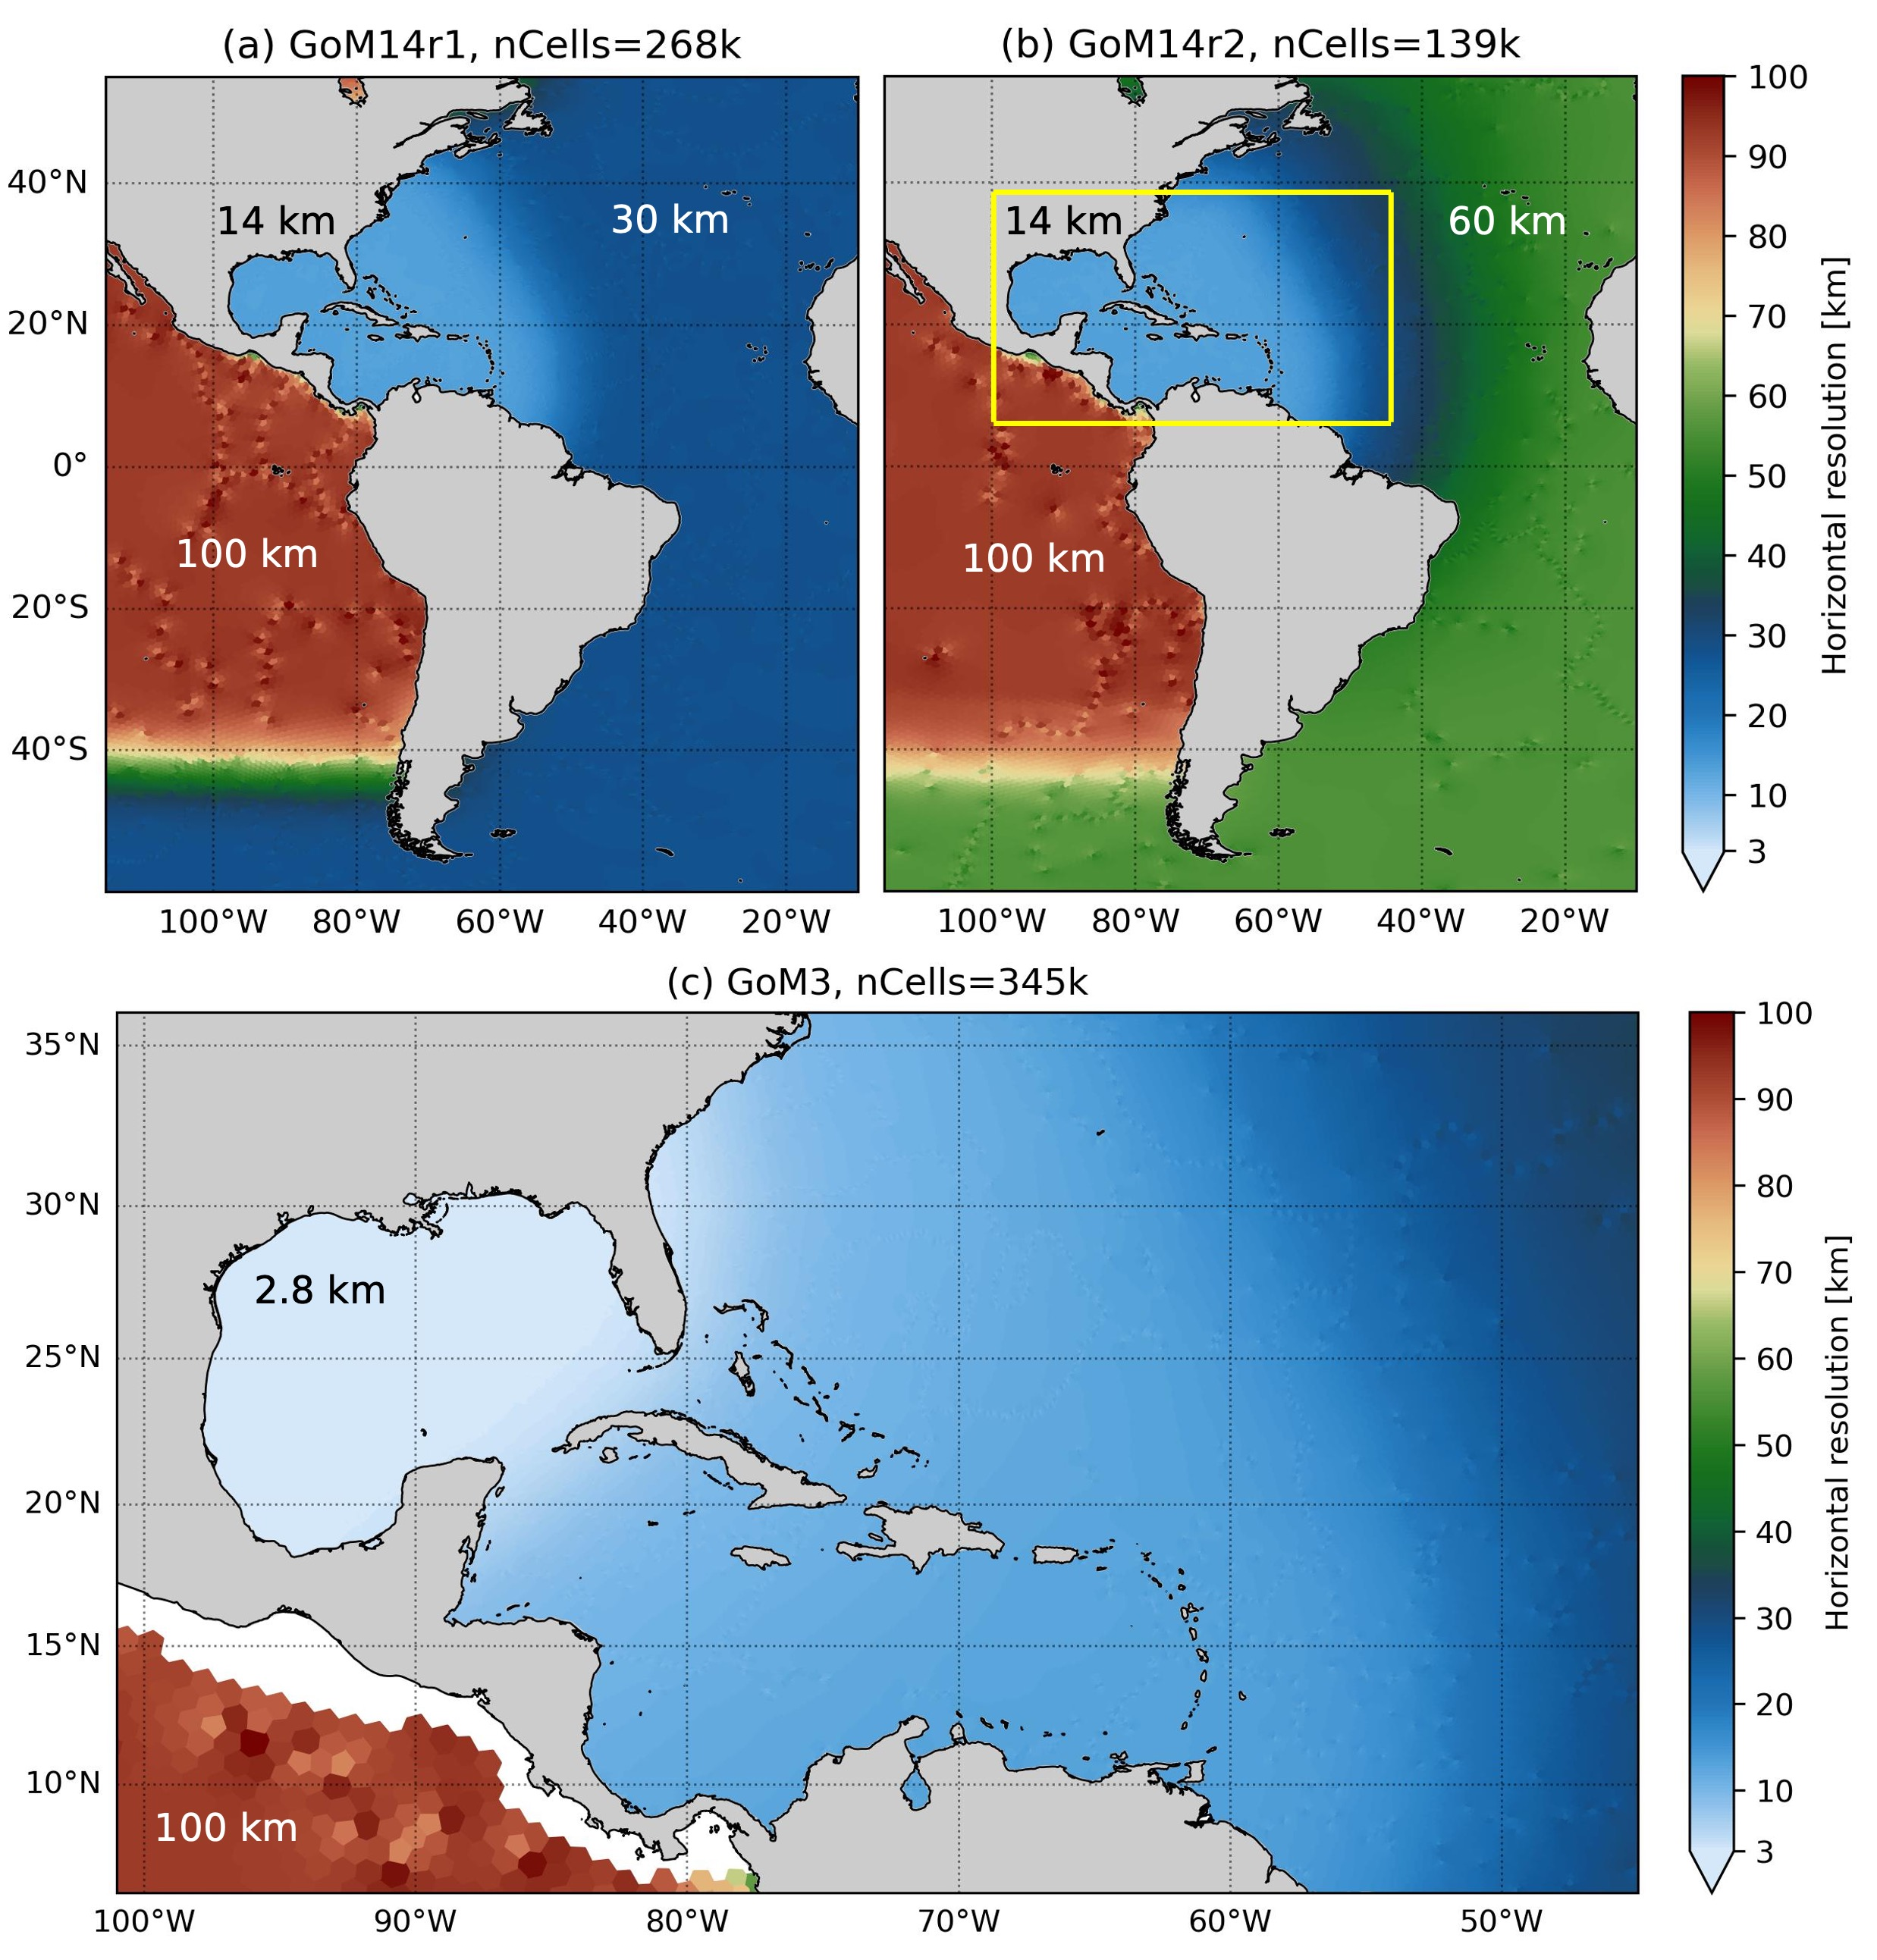
\includegraphics[width = \textwidth]{figures/scgsr/gom_resolutions.jpg}}
    \caption{Horizontal grid cell resolution for GoM14r1 (a), GoM14r2 (b), and GoM3 simulations (c). The broader Pacific and Indian Oceans (not shown) are set to a horizontal resolution of 100 km.}
    \label{fig:mesh_overview}
\end{figure}

First, the TXLA shelf has been the subject of intense observational and modeling efforts due to seasonal occurrences in hypoxia and the 2010 \textit{Deepwater Horizon} oil spill \citep{bianchi2010science,  dukhovskoy2021development, Zhang_2012_forecast}, which allows for an accurate assessment of the fidelity of MPAS-O in representing GoM coastal processes. The MPAS-O simulations developed here are directly compared with the validated ROMS-based TXLA model, which has been run at submesocale eddy-permitting resolution ($\mathcal{O}$(1.5 km)) in early iterations used for hypoxia studies \citep{ruiz2021small, Zhang_2012_numerical}, submesoscale eddy-resolving resolution ($\mathcal{O}$(300 m)) in a two-way nested iteration to aid observational campaigns focused on submesoscale fronts \citep{Qu_2022_NIW, Schlichting23}, and front-refined resolution simulations ($\mathcal{O}$(100 m)) used to understand processes identified from the observations \citep{qu2022rapid}. Second, circulation patterns over the shelf exhibit pronounced seasonal variability, allowing us to assess MPAS-O's representation of submesoscales under variable forcing, a challenging test case. Third, the TXLA shelf features a wind-driven inner shelf circulation inshore of the 50 m isobath, whereas interactions between the plume and loop current (LC) eddies influence the outer shelf circulation \citep{zhang2014wind}. Therefore, the location and gradient of the transition region to a lower grid resolution outside the GoM deserves special consideration so that a realistic loop current is produced.

In the following, we describe the mesh generation process, changes to river forcing, and tuning of key subgrid-scale parameterizations that were shown to have a significant impact on the permitted submesoscales' characteristics. We present preliminary analysis of the GoM3 meshes and compare the representation of surface fronts and the M/A River plume structure with existing TXLA model output. We discuss the strengths and limitations of the current MPAS-O code base that may be used to inform future capability development and regionally refined applications. Finally, we conclude with a discussion of MPAS-O's utility for coastal refined simulations relative to a model nesting approach and discuss future work.

\section{Submesoscale variability in the GoM}
Here we will give a brief overview of the life cycle and seasonal variability of submesoscales over the TXLA shelf and broader GoM to contextualize model results. As reviewed in previous studies \citep{McWilliams_2016, taylor2023submesoscale}, the lateral density (buoyancy) gradient is a key variable that modulates submesoscale generation. Over the TXLA shelf, lateral density gradients are dominated by salinity variations due to freshwater input from the M/A rivers \citep{Hetland_2017}. While, over the broader GoM, density gradients are modulated by both mesoscale eddies shed from the LC and freshwater input from the M/A Rivers \citep{bracco2019mesoscale, liu2021submesoscale}. Submeoscales extract energy from the mixed layer by releasing potential energy stored in the lateral density gradients. The strength of these submesoscales is then closely related to the mixed layer depth because a deeper mixed layer allows for more potential energy to be released \citep{boccaletti2007mixed, fox2008parameterization}. In the open ocean, submesoscales tend to follow a seasonal cycle where they are stronger in winter due to a deeper mixed layer and weaker in summer \footnote{The mixed layer depth is shallower on average in summer due to increased radiative heating.} \citep{callies2015seasonality}. 

In the TXLA shelf region, submesoscales are primarily generated by mixed layer instabilities and surface frontogenesis, or the sharpening of horizontal density gradients \citep{hoskins1982mathematical, mcwilliams2021oceanic}. Frontogenesis is thought to be a primary generation mechanism in the Louisiana Bight west of Southwest Pass and M. River jet east of Bird's Foot \citep{Barkan_2017, wang2021structure}, whereas baroclinic mixed layer instabilities dominate submesoscale generation west of Atchafalaya Bay \citep{Hetland_2017, Schlichting23}. During summer months (JJA), M/A river discharge relaxes relative to spring and a weakly up-coast diurnal land-sea breeze causes freshwater to pool over the shelf, which creates baroclinic instabilities that develop into a rich submesoscale eddy field \citep{Hetland_2017, Kobashi_2020, Schlichting23}. During nonsummer months, downwelling-favorable winds, higher relative river discharge, and cold front passages reduce the stratification created during summer and produce a bottom-advected plume that suppresses eddy formation \citep{hetland2012integrated, zhang2014wind}.

In the broader GoM, \citet{barkan2017submesoscalepart2} showed river discharge can enhance or suppress submesoscales forming near LC eddies over the northern continental shelves. River discharge can energize LC eddy (LCE) fronts by providing a source of brackish water, or suppress them by increasing near-surface stratification. River discharge rates are generally lower during winter (DJF), so submesoscales are generally thought to be more prevalent in the winter than summer. In addition, "submesoscale soup" forms year-round in the eastern GoM and over the Florida shelf, consisting of chaotic fronts, filaments, and eddies \citep{Barkan_2017, liu2021submesoscale}. Given the seasonal differences and the strong freshwater river plume control in both regions, our analysis of the MPAS-O simulations will mostly focus on the surface structure of the M/A river plume and basic estimates of seasonal variability over the TXLA shelf and broader GoM. 

\section{Model setup} \label{sec:coupled_setup}
\subsection{TXLA ROMS model}
The iterations of the TXLA ROMS model are described in previous studies \citep{Kobashi_2020, qu2022rapid, Schlichting23}. Here, we review the dynamical core, discretization methods, subgrid-scale parameterizations, and model forcing so they can be compared with the coupled MPAS-O simulations. The simulations here use the Coupled Ocean-Atmosphere-Wave-Sediment Transport Model \citep{Warner_2010} version of ROMS.

ROMS uses the incompressible, hydrostatic and Boussinesq approximations to solve the primitive equations on a structured, curvilinear Arakawa C-grid \citep{Arakawa_1977, shchepetkin2005regional}. ROMS uses a split explicit time stepping scheme with several numerical methods available for the stepping the baroclinic and barotropic modes. In the simulations presented here, the baroclinic mode is stepped with a third order Adams Bashforth scheme and the barotropic mode is stepped with a third order Adams Moulton-Leapfrog scheme. The tracers are stepped with a trapezoidal leapfrog scheme. Momentum advection is computed using a third order upwind scheme and tracer advection is computed with the multidimensional positive definite advection transport algorithm \citep{Smolarkiewicz_1998}. The simulations here use an 80 s baroclinic timestep and a two s barotropic timestep. 

The TXLA model domain in shown in Fig. 1 of \cite{Schlichting23}, with horizontal resolution varying from 0.6 km close to the coast to 3.7 km near the outer continental slopes. Inshore of 100 m depth, the model resolution is approximately 1.5 km for the analysis region in this paper, which is the location of the child grid used in a nested application \citep{Schlichting23}. The model uses terrain following vertical coordinates with 30 vertical layers stretched near the surface to better resolve the surface boundary layer. The mean vertical resolution in the top one m of the water column (where the M/A plume is most prominent) is approximately 38 cm in the region of interest. The minimum water depth $h_{min}$ is 5 m. 

The TXLA model uses the $k-\omega$ vertical mixing scheme, a two equation model configured as part of the Generic Length Scale library \citep{umlauf2003extending, Warner_2005}. The model uses a geopotential aligned horizontal mixing scheme with constant values scaled to the grid size \citep[see Section 3.2 of ][]{Schlichting23}. The open boundary is forced by Gulf of Mexico HYCOM as described in \citep{Zhang_2012_forecast}. ERA-interim datasets are used to provide surface fluxes \citep{Dee_2011} and river forcing is provided daily by USGS streamflow data for nine regional rivers. Although model snapshots are saved hourly, they are subsampled each day so sampling frequency matches MPAS-O output. Further ROMS documentation is available at \url{https://github.com/kshedstrom/roms_manual/blob/master/roms_manual.pdf}.

\subsection{The model for prediction across scales-ocean (MPAS-O)}
MPAS-O solves a mimetic finite volume discretization of the primitive equations, which makes use of the incompressible, hydrostatic, and Boussinesq approximations to solve prognostic equations for momentum, thickness (volume), and tracers. A key difference relative to ROMS is that MPAS-O solves a vector invariant form of the momentum equations presented in vorticity-kinetic energy form such that momentum advection is expressed as the sum of the gradient of the kinetic energy and the vector product of velocity and vorticity. This approach is required to guarantee the consistent and compatible evolution of mass, velocity, and potential vorticity for arbitrarily structured Arakawa C-grids \citep{Arakawa_1977, ringler2010unified}. The simulations presented here used a second order Adams-Bashforth split explicit time stepping method. Tracer advection is computed with a monotonic, third order flux-corrected transport scheme described in \cite{skamarock2011conservative}. 

Mesh generation is performed using the JIGSAW library \citep{engwirda2017jigsaw}. As \cite{hoch2020mpas} summarizes, JIGSAW incrementally creates an unstructured mesh by first creating a conforming Voronoi/Delaunay tessellation, which is optimized using Optimal Delaunay Tessellation techniques. As a result, the final mesh can consist of triangular and polygonal cells that guarantee a locally orthogonal C-grid staggering that satisfies the requirements detailed in \cite{ringler2010unified}. The simulations presented here use a geopotential-aligned $z^*$ vertical coordinate that oscillates with the sea surface height, designed within an Arbitrary Lagrangian-Eulerian framework \citep{Petersen_2015, griffies2020primer}. 

The vertical mixing scheme is the K-Profile Parameterization \citep[KPP, ][]{large1994oceanic, van2018kpp} configured as part of the CVMix library (\url{https://cvmix.github.io/}). The Gent-McWilliams (GM) thickness advection scheme \citep{gent1990isopycnal} is used to parameterize horizontal transport by mesoscale eddies. The GM scheme is applied to grid cells larger than 30 km and linearly tapered to zero by 20 km. GM is used in conjunction with an isoneutral-aligned diffusion tensor described by \citep{redi1982oceanic} that is tapered similarly to GM. Coefficients used for the GM ($\kappa_{GM}$) and Redi ($\kappa_{redi}$) schemes for all GoM simulations are shown in Tab. \ref{tab:mpaso_sims}. Harmonic ($\nu_2$) and biharmonic ($\nu_4$) lateral viscosity are applied to the momentum equations and scaled to the grid size as 
\begin{equation}
    \nu_2 = \nabla_0^4 \, [\textrm{m}^2 \textrm{s}^{-1}] \frac{\Delta x}{30 \, [\textrm{km}]} \, ,
\end{equation}
\begin{equation}
    \nu_4 = \nabla_0^4 \, [\textrm{m}^4 \textrm{s}^{-2}] \left(\frac{\Delta x}{30 \, [\textrm{km}]}\right)^3 \, ,  
\end{equation}
where $\nabla_0^2$ and $\nabla_0^4$ are the background coefficients for $\nu_2$ and $\nu_4$, respectively, and $\Delta x$ is the horizontal cell width. No explicit horizontal diffusion is applied to the tracers. 

\begin{table}[t] 
\caption{Key parameters used in the GoM refined simulations as defined in text. $^*$ The mean value of $\nabla_0^4$ used in the GoM3r1 simulation is 2.35e10 [m$^4$s$^{-2}$]. $^+$ The mean value of $\nabla_0^4$ used in the GoM3r2 simulation is 3.25e10 [m$^4$s$^{-2}$].} \label{tab:mpaso_sims}
\begin{center}
\begin{tabular}{ccccc}
\hline
Variable & GoM14r1 & GoM14r2 & GoM3r1 & GoM3r2 \\
nCells [$10^5$] & 2.68 & 1.39 & 3.45 & 3.45 \\
$h_{min}$ [m] & 20 & 20 & 20 & 10 \\
$z_{lay}$ [m] & 64 & 64 & 64 & 128 \\
$z_{min}$ [m] & 10 & 10 & 10 & 2 \\
DT [min:s] & 10:00 & 10:00 & 02:30 & 02:30 \\
BTR\_DT [min:s] & 00:15 & 00:15 & 00:07.5 & 00.07.5 \\
$\nabla_2^0$ [m$^2$s$^{-1}$] & 462 & 462 & 66.7 & 66.7 \\
$\nabla_4^0$ 10$^{10}$[m$^4$s$^{-2}$] & 1.2 & 1.2 & 2.0-3.5$^*$ & 2.0-4.5$^+$ \\
$\kappa_{GM}$ [m$^2$s$^{-1}$] & 600 & 600 & 300 & 300 \\
$\kappa_{redi}$ [m$^2$s$^{-1}$] & 400 & 400 & 300 & 300 \\
\hline
\end{tabular}
\end{center}
\end{table}

In addition, the simulations are forced by Japanese 55-year reanalysis \citep[JRA-55, ][]{kobayashi2015jra}, which provides surface momentum, heat, and freshwater fluxes and river runoff fluxes at 0.25$^\circ$ resolution every three hours. Tidal forcing is not included because it is still under development for baroclinic applications \citep{barton2022global}. We do not anticipate this to be a significant source of bias for representation of the M/A river plume because tides are weak over the region \citep{DiMarco_1998} and excluded from the TXLA model. The coupled GoM simulations are described in the next section. Further MPAS-O documentation may be found in \cite{petersen2018mpas}.

\subsection{MPAS meshes and coupled simulations}
A primary factor governing our design of the MPAS meshes and coupled simulations is the target simulation length of 11 years (2000-2011), which allows for an estimate of submesoscale variability in the broader GoM and TXLA shelf. We focused on 2000-2010 because we have existing TXLA model output to compare to and there is strong interannual variability among various forcing mechanisms \citep[see Tab. 2 of ][]{forrest2011multivariable}. We configured the GoM simulations as an E3SM ``G case" such that MPAS-O is coupled with an active version of MPAS Sea Ice \citep{petersen2019evaluation, turner2022mpas}, while all other components are driven by data. The outer TXLA shelf circulation is modulated by interactions with LCEs, which are shed stochastically from the LC in roughly three to 17 month intervals \citep{oey2005loop}. High fidelity representation of the LC requires realistic representation of the Atlantic Meridional Overturning Circulation (AMOC). As reviewed by \cite{richardson2005caribbean}, the LC structure is determined by the northward flowing transport via the Caribbean current, which is forced by the North Brazilian and Equatorial currents. These larger-scale currents are affected by the representation of sea ice in the Southern Ocean on subdecadal timescales, thereby necessitating the use of MPAS Sea Ice.

We targeted a 3 km resolution within the GoM, which is slightly higher resolution than models (e.g. GoM-HYCOM, 1/25$^\circ$, \url{https://www.hycom.org/data/goml0pt04}) that typically provide open boundary forcing for shelf-scale regional models. Previous studies that focused on submesoscale variability in the GoM used 1.5 km resolution or higher \citep{barkan2017submesoscalepart2, bracco2019mesoscale, liu2021submesoscale}. While we plan to design a 1.5 km mesh in the future, 3 km was deemed more practical because it allowed us to develop trial simulations more efficiently that were needed to address two aspects of model configuration unrelated to horizontal resolution. The first was the vertical grid; MPAS-O experienced stability issues (discussed later) near the M/A discharge points when run at high vertical resolution ($<$2 m layers). The second was the implementation of the river forcing; in E3SMv2, rivers are spread in an un-physical way for stability reasons. Ideally, river forcing should be treated as point sources as done in regional models like ROMS. However, this was not implemented in E3SM because the model was not initially developed to simulate coastal processes and changing this would require a complete overhaul of the code. Both aspects are discussed further in the following sections. 

The simulations are first spun up in stand alone (just constant atmospheric forcing) for one month with Rayleigh damping to reduce grid scale noise caused by initialization shock and surface gravity waves \cite{petersen2018mpas}. This allows us to reach a target timestep for the coupled simulations that scales proportionally with the smallest cell width (1 min timestep / 1 km cell width). For example, a 150 s baroclinic and 7.5 s barotropic timestep were used in the GoM3 simulations because the smallest grid cell is approximately 2.5 km.

While many initial mesh configurations were tested in the design process (some of which is detailed below), final analysis was performed on two GoM3 simulations with low (10 m layers) - and medium (2 m layers) resolution vertical meshes (GoM3r1, GoM3r2; Tab. \ref{tab:mpaso_sims}). Target vertical resolution was 0.5 m layers to be comparable to the TXLA model. GoM3r1 was analyzed despite the low vertical resolution because the representation of submesoscales in the broader GoM is less dependent on vertical resolution compared to the TXLA shelf and it seldom experienced stability issues. Following preliminary analysis, we restricted run time to two years (2000-2001) following a two year spinup, which allowed for a baseline estimate of seasonal variability in the GoM. A two year spinup is comparable to previous studies focusing on meso- and submesoscale dynamics in the GoM and TXLA shelf \citep{Barkan_2017, Kobashi_2020}. Simulations were run for only two years because they did not produce a submesoscale eddy field over the shelf.  In addition, all ``trial simulations'' used to develop the GoM3 meshes were initialized in 1958 (the first year of JRA forcing).

We ran the GoM3 simulations on 32 nodes with 128 processes per node. High frequency output of key two dimensional variables (e.g. surface active tracers, surface relative vorticity) were saved daily. Three dimensional variables were saved monthly.  

\subsubsection{Horizontal meshes}
The final mesh configurations used in the analysis portion of this study have a relatively course resolution in much of the global ocean, likely too coarse to perform climate length simulations with any accuracy or defend a fully coupled configuration with the other active components of E3SM. This decision was justified for two reasons: 1) the target simulation length is decadal, and the time scale of the Pacific and Indian Ocean currents affecting the larger-scale ocean state within the GoM is much longer, negating a need for an accurate Pacific or Indian ocean state, 2) model tuning is a goal of this project, and higher resolution outside the region of interest increases computational cost, which slows the rate of model tuning experiments. Regarding the latter, the quality of resolved submesoscale features is extremely sensitive to horizontal mixing coefficients and is discussed later. Thus, we used 100 km resolution in the Pacific and Indian Oceans to minimize computational resources spent outside the region of interest. 

We tested two horizontal mesh configurations (Fig. \ref{fig:mesh_overview}) that relax resolution to 30- and 60 km in the broader Atlantic and Southern Oceans, denoted as GoM14r1 and GoM14r2, respectively. Both meshes used 14 km resolution within the GoM, southern Sargasso Sea, and Caribbean Seas. The 14 km mesh was used instead of three km for the GoM because the 14 km mesh allowed us to more efficiently assess the larger-scale currents that affect the LC. The transition from high to low resolution regions used weighted $\tanh$ functions similar to Eqs. 3-4 of \cite{hoch2020mpas}. The transition from 100-60 km (30 km) used a transition width of 1000 km with no offset from the coast. GoM14r1 (Fig. \ref{fig:mesh_overview} a) used a transition width of 1000 km for the 30- to 14 km regions with a 1000 km offset from the coast. GoM14r2 (Fig. \ref{fig:mesh_overview} b) used the same transition width from 100-60 km but includes an additional refinement from 60-30 km that is 3000 km wide and offset 2500 km from the coast. The transition from 30-14 km is the same as GoM14r1. GoM14r1 had nearly twice as many cells (268 thousand) as GoM14r2 (139 thousand), suggesting a 30 km Atlantic and Southern Ocean placed over half the number of cells outside of the region of interest. We provide details of the GoM3 mesh below after analysis of the GoM14 simulations. 

A two year simulation length is insufficient to properly compare biases with the standard and high resolution E3SM test cases \citep{golaz2022doe, caldwell2019doe}. However, we were able to do a quantitative comparison between the GoM14 meshes and get a sense of scale of their differences, especially in the Atlantic Ocean, and a preliminary estimates of model biases. 

We compared GoM14r1 and GoM14r2 using MPAS-Analysis (\url{https://mpas-dev.github.io/MPAS-Analysis/stable/index.html}), a post processing package designed for analysis of coupled E3SM simulations. We present outputs of several analysis tasks: 1) the time- and zonally-averaged barotropic Atlantic MOC streamfunction $\psi$ (Fig. \ref{fig:moc}), 2) time- and zonally-averaged global meridional heat transport (MHT, Fig. \ref{fig:mht}), and 3) time series of inflowing volume transport through the Antilles Archipelago (Fig. \ref{fig:antilles}). The MOC streamfunction was used to qualitatively examine the vertical structure of the meridional volume transport in the Atlantic Ocean. The MHT was directly compared to observations \citep{trenberth2001estimates} and provides an example of tracer transport bias resulting from the low resolution regions. The Antilles inflow may be compared directly against observations and provides larger-scale forcing for the LC. The metrics discussed above were used to determine whether 60 km resolution in the Atlantic is justifiable relative to 30 km resolution. Details of the computations may be found in the MPAS-Analysis documentation. 

\begin{figure}[h]
\centerline{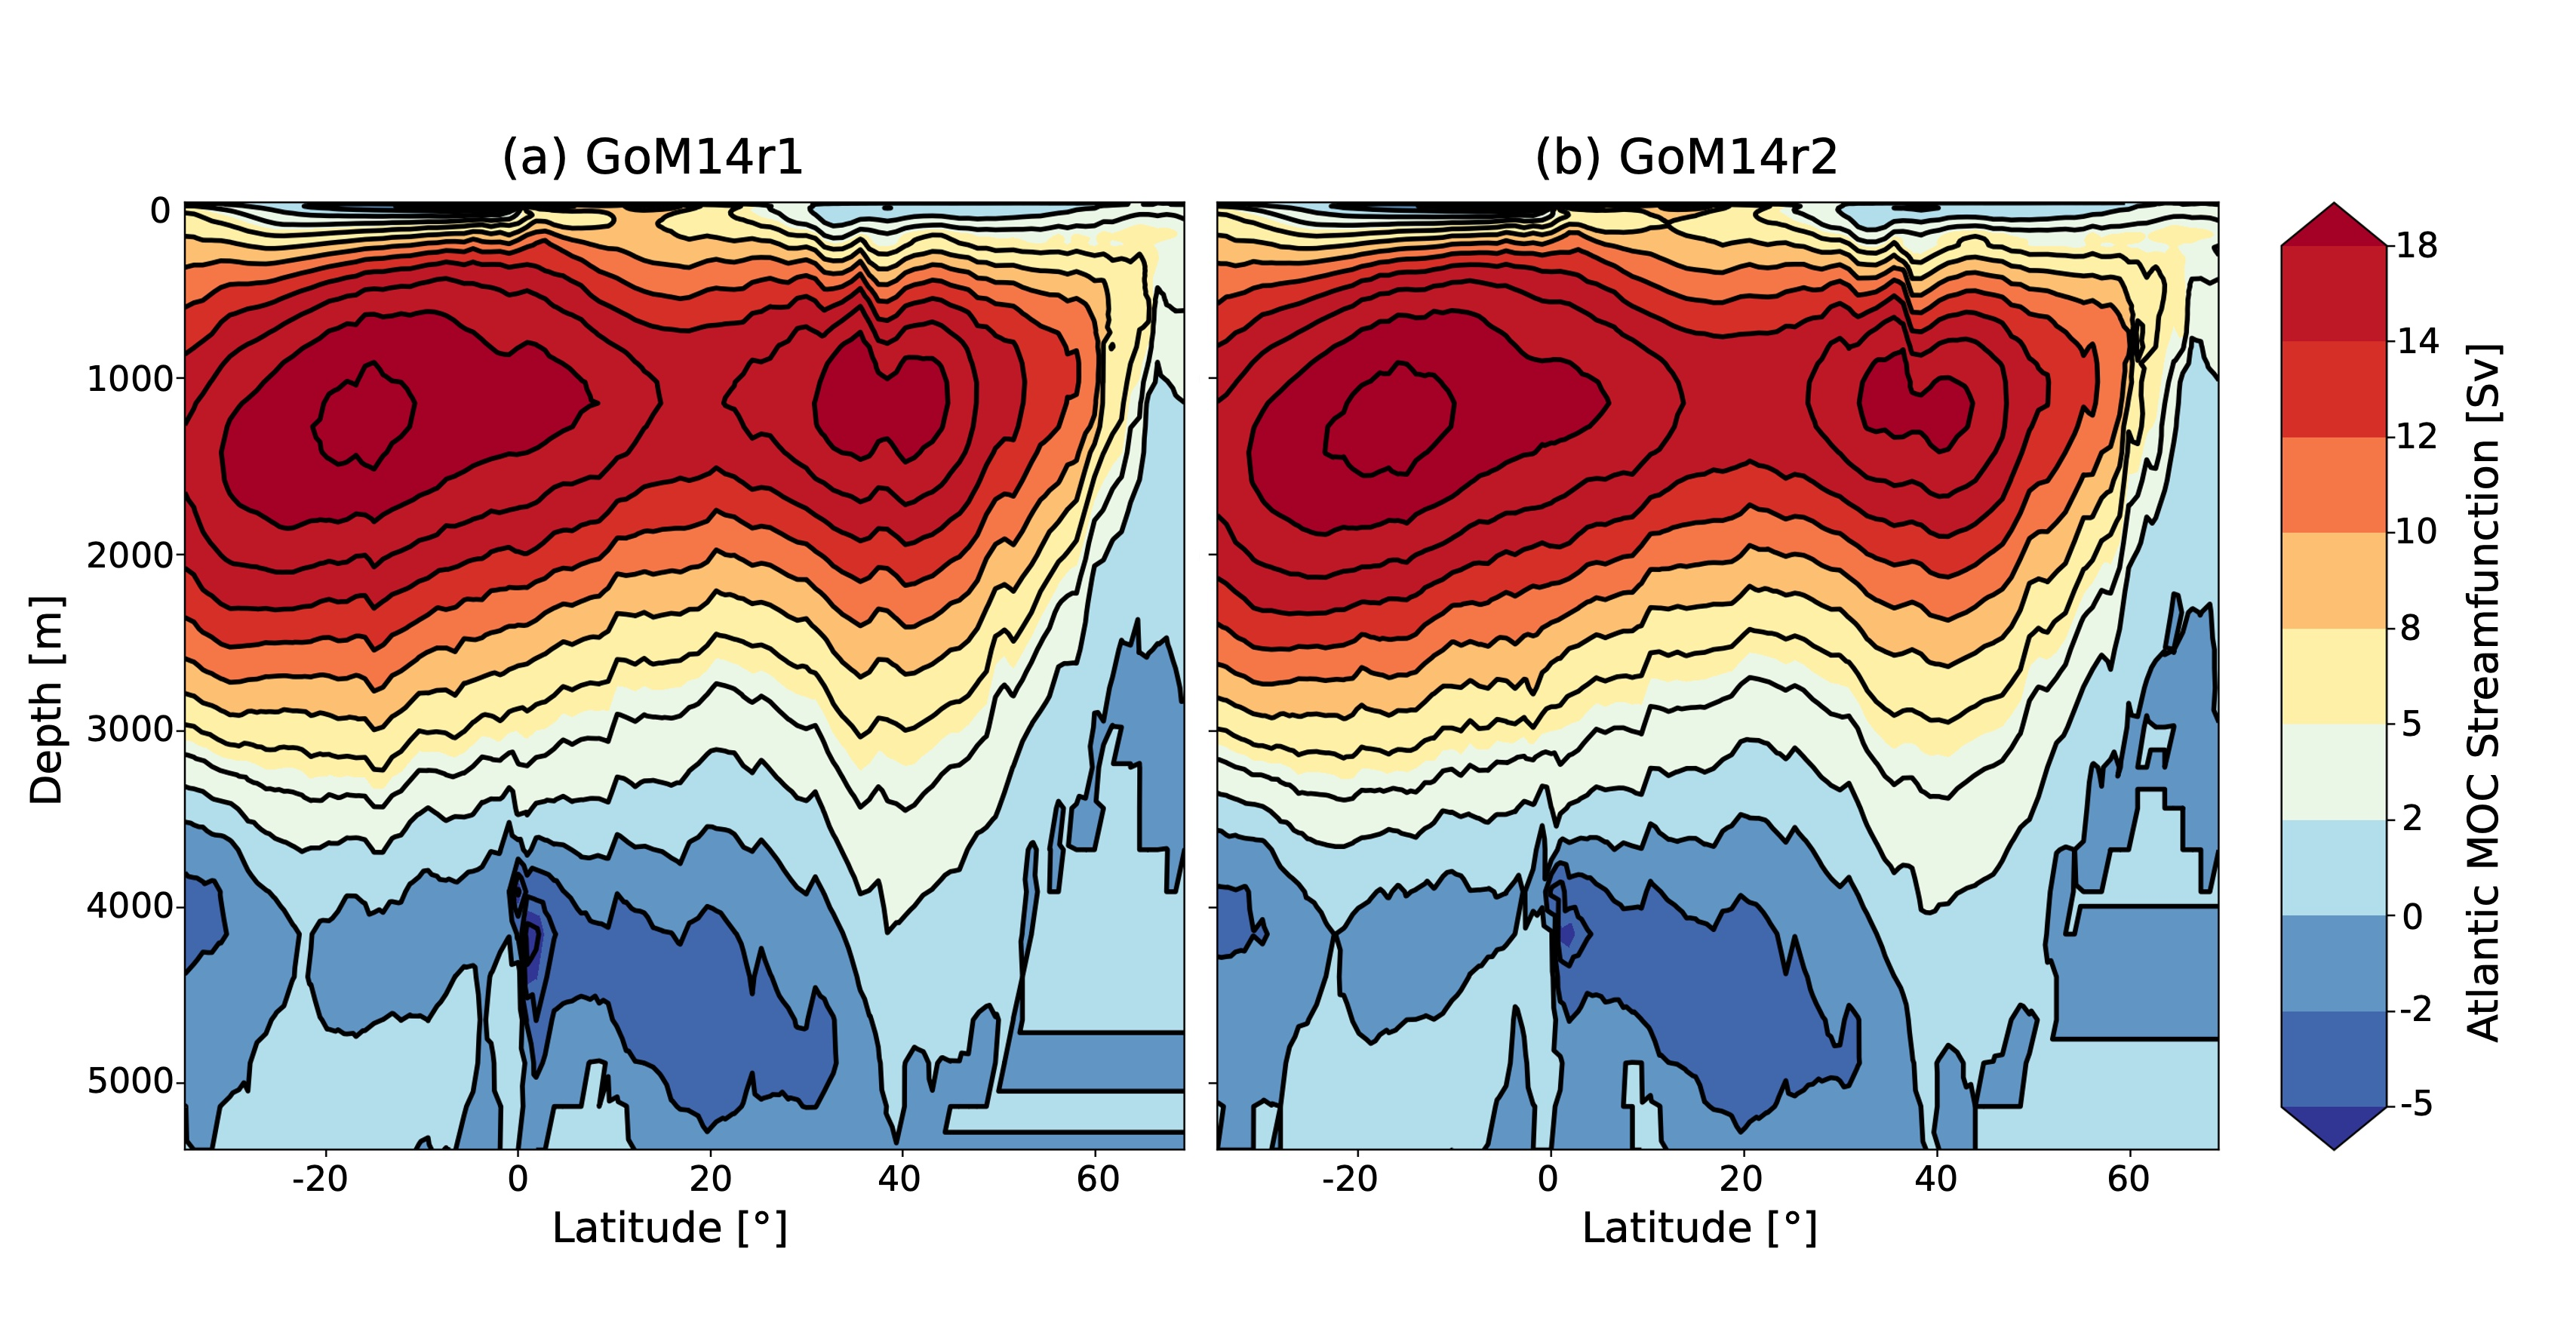
\includegraphics[width=\textwidth]{figures/scgsr/atlantic_moc.jpg}}
    \caption{Zonally-averaged barotropic streamfunction for the Atlantic meridional overturning circulation for GoM14r1 (a) and GoM14r2 (b) integrated over the two year simulation. Contours are overlaid every Sv.}
    \label{fig:moc}
\end{figure}

\begin{figure}[h]
\centerline{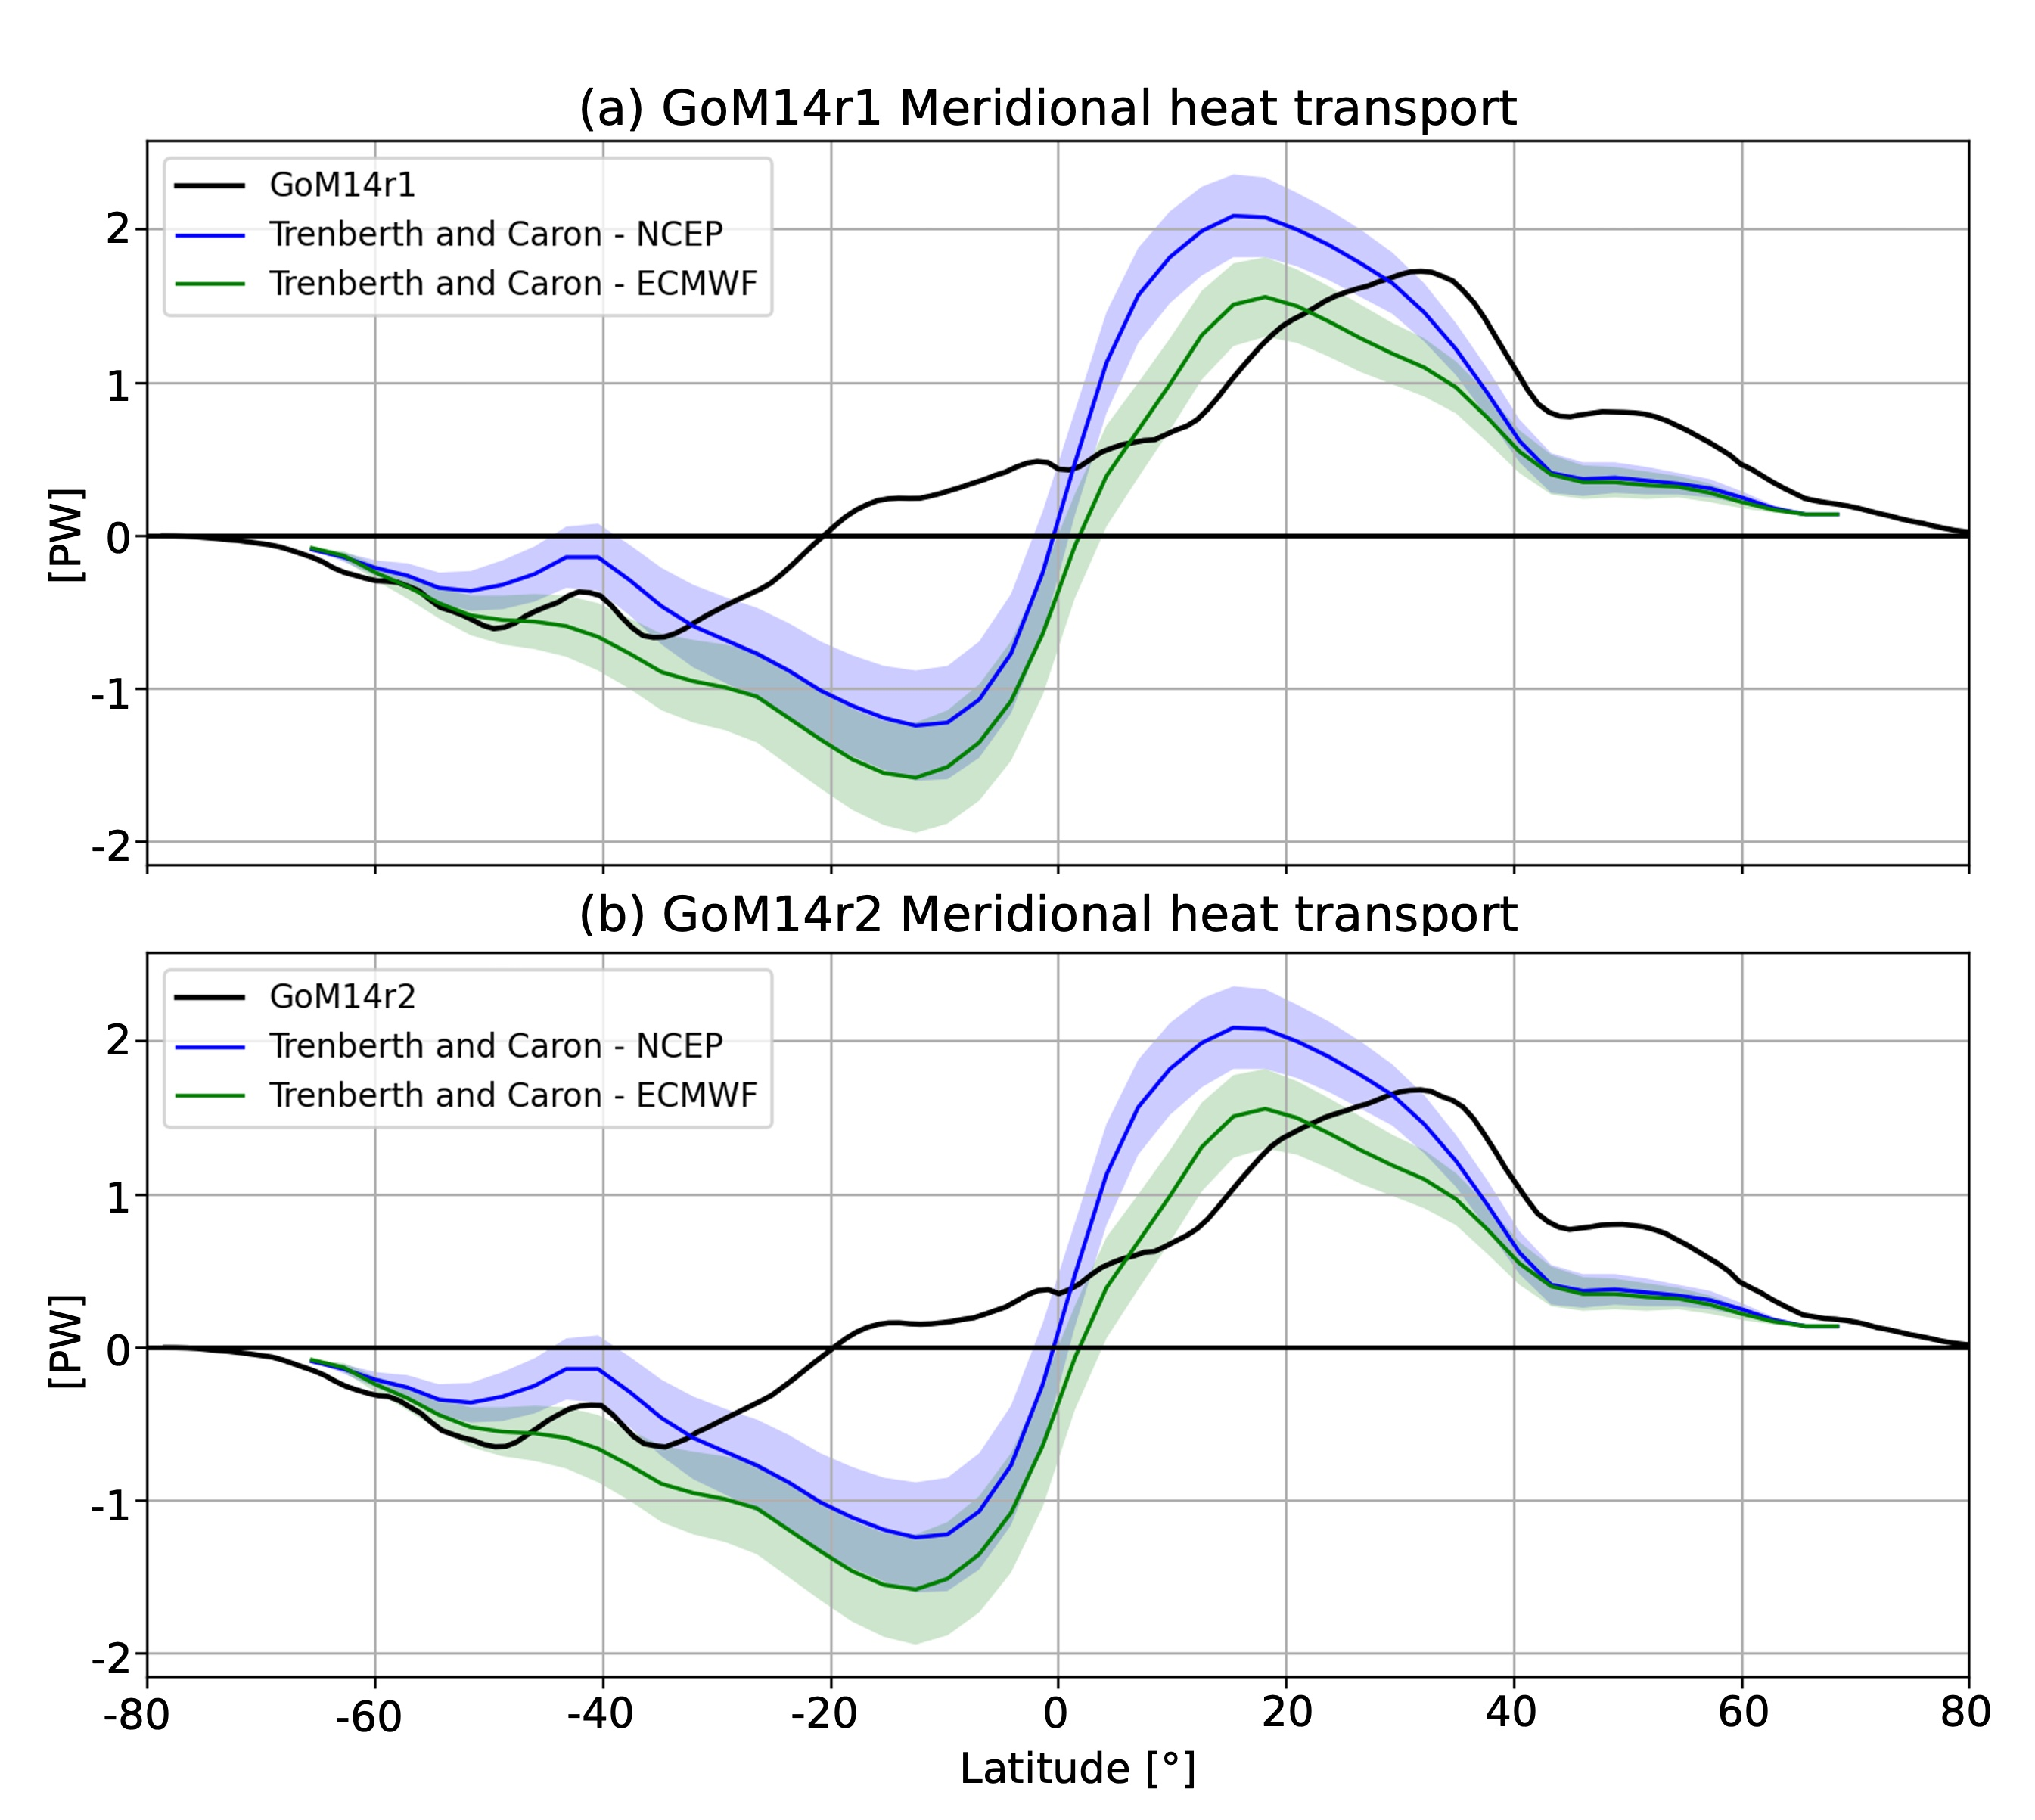
\includegraphics[width=0.9\textwidth]{figures/scgsr/mht_gom14.jpg}}
    \caption{Zonally-averaged MHT for GoM14r1 (a) and GoM14r2 (b) averaged over the two-year simulation relative to observations \citep[see][]{trenberth2001estimates}. The shaded areas represent one standard deviation about the mean of the observations.}
    \label{fig:mht}
\end{figure}

\begin{figure}[h]
\centerline{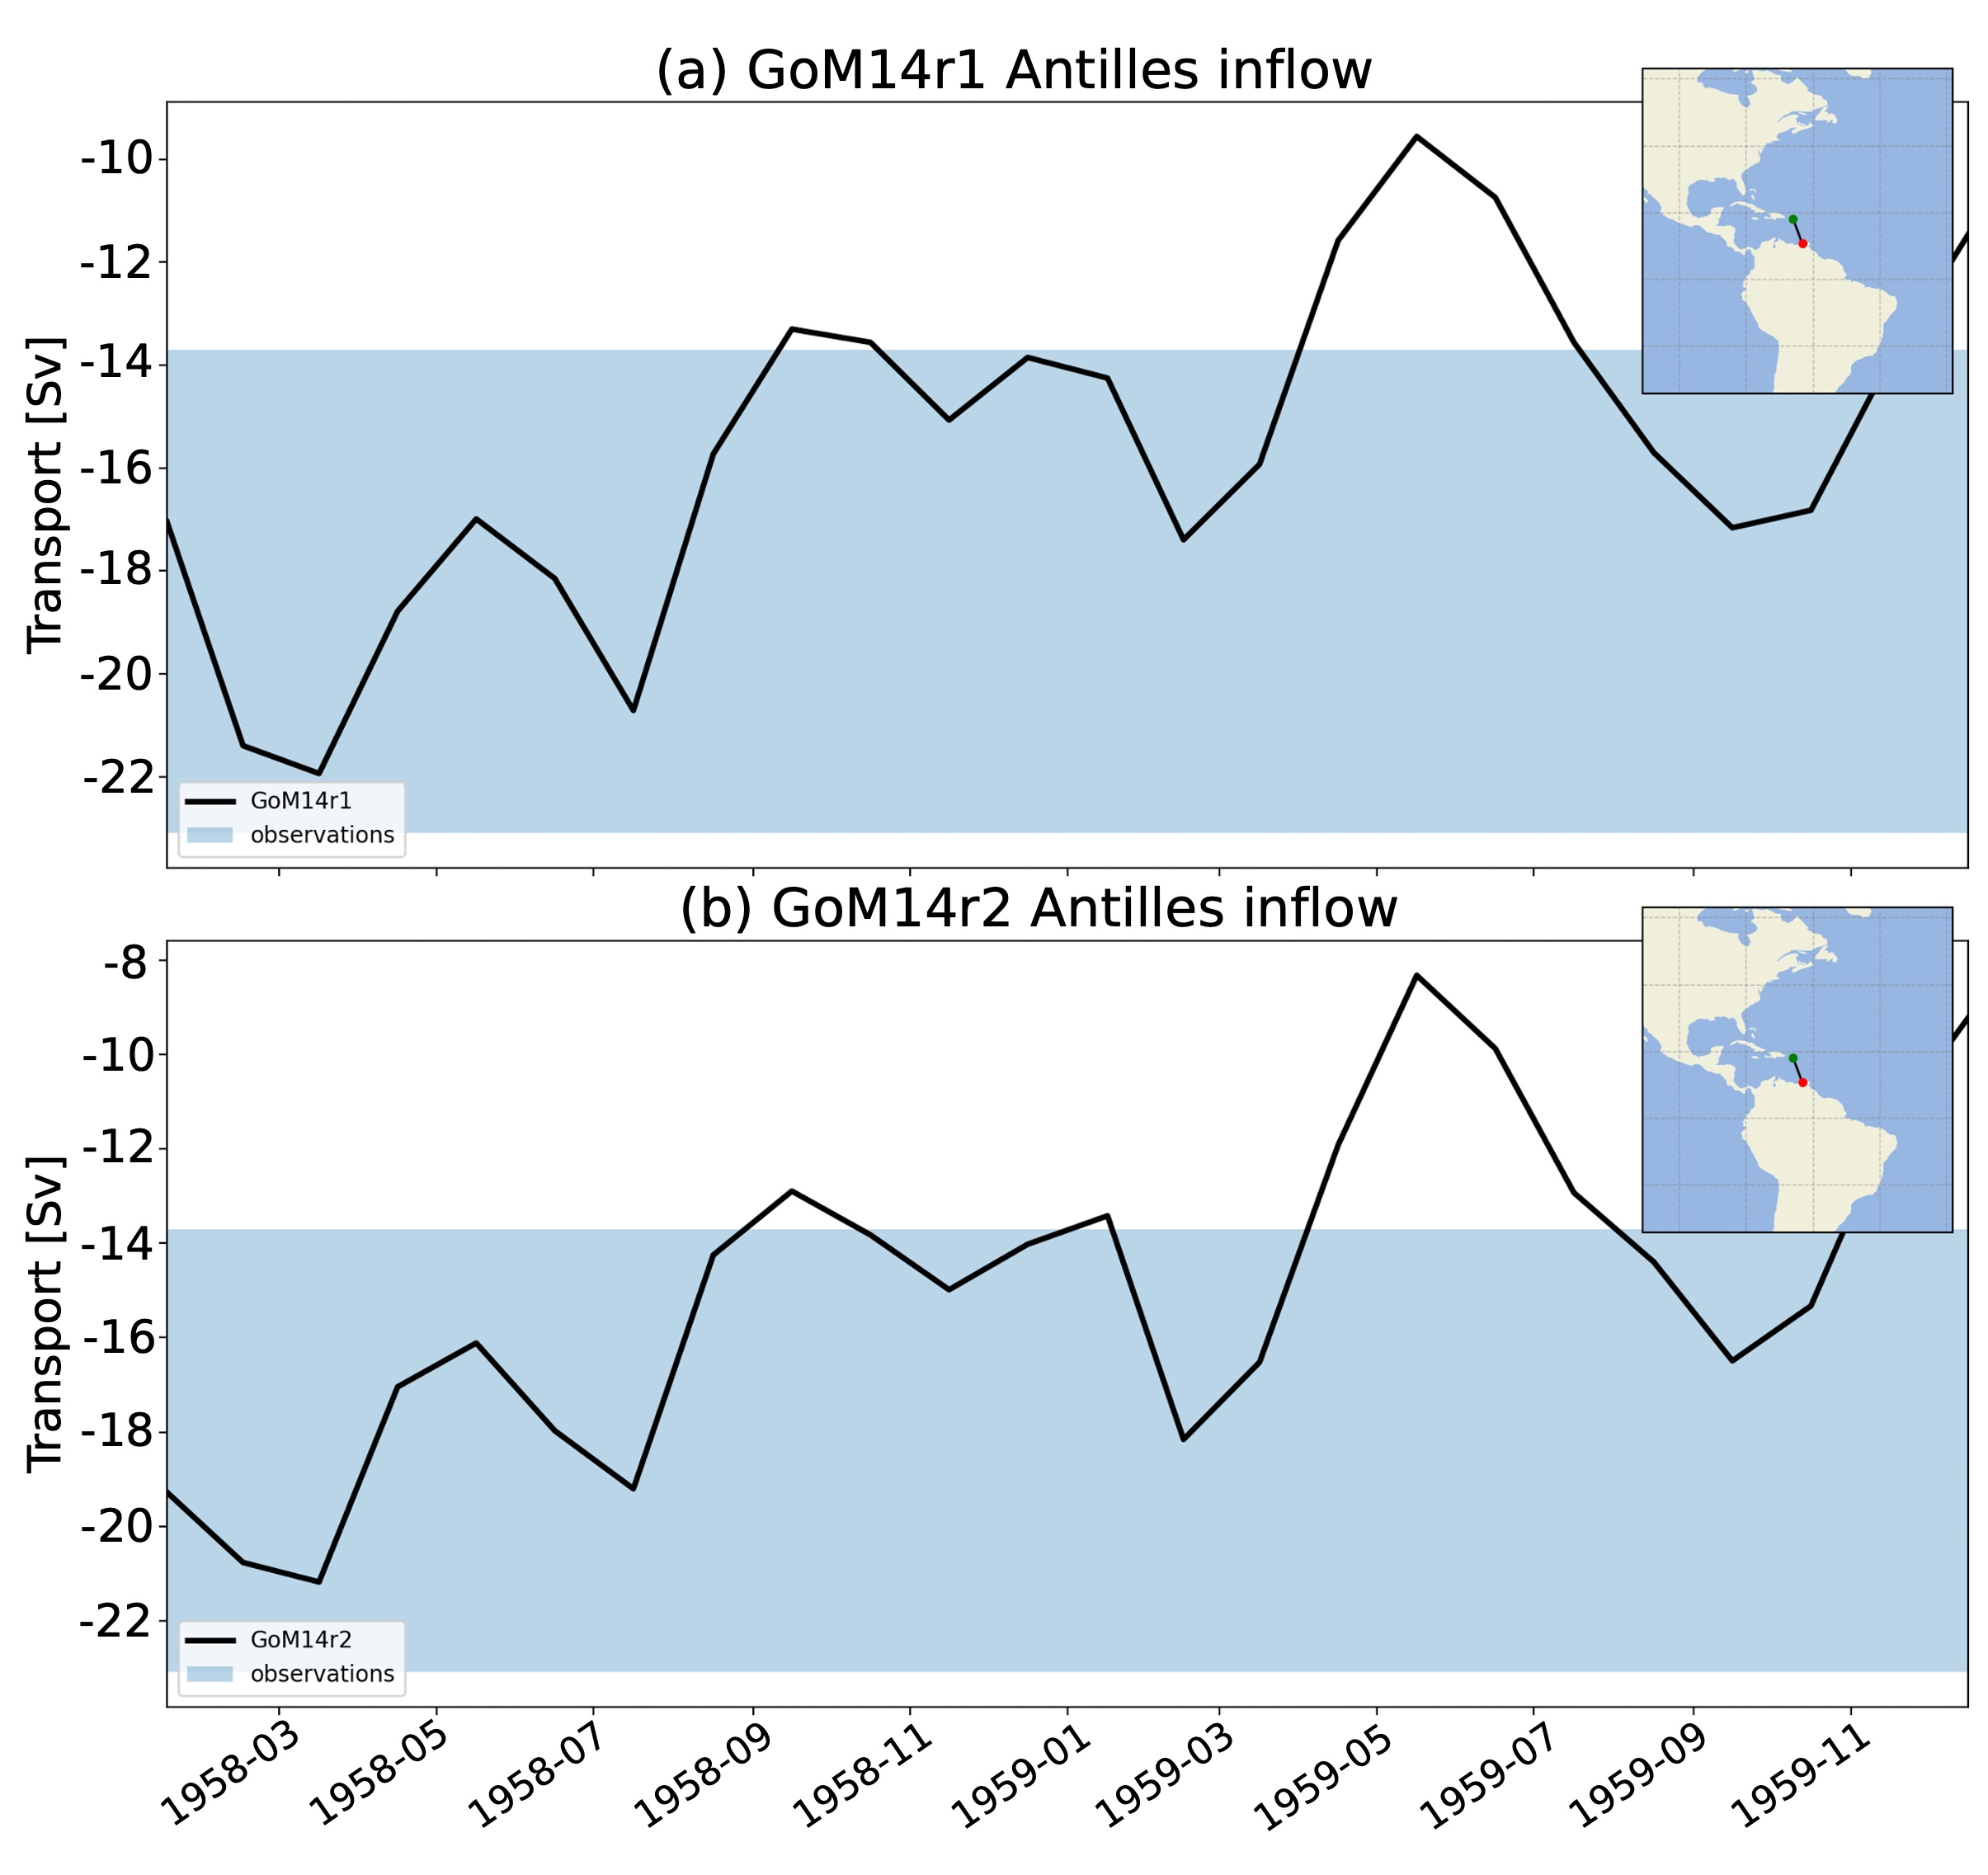
\includegraphics[width=0.8\textwidth]{figures/scgsr/antilles_inflow.jpg}}
    \caption{Time series of inflowing volume transport through the Antilles Archipelago for GoM14r1 (a) and GoM14r2 (b) relative to observations, which are shaded by one standard deviation on either side of the mean value.}
    \label{fig:antilles}
\end{figure}

The MPAS-Analysis results suggest the differences between GoM14r1- and -2 are marginal in the region of interest. The MOC streamfunctions are qualitatively similar south of 40$^\circ$N. North of 40$^\circ$N, GoM14r2 exhibits stronger southward flow ($\psi<0$) below 2000 m depth and weaker northward flow above 2000 m due to coarser resolution. The zonally-averaged MHT transport demonstrates the model biases exceeding 1 PW in the subtropics in both hemispheres and 0.5 PW at midlatitudes of the northern hemisphere. We assume these biases are caused by two factors: 1) Use of JRA-55 for atmospheric forcing instead of coupling with MPAS-Atmosphere, and 2) the 100 km resolution in the Pacific and Indian Oceans. Further investigation these biases is beyond the scope of this study, however, it suggests the GoM3 mesh is likely unsuitable for long term climate simulations. In addition, the Antilles inflow for both meshes are quantitatively similar. However, the transport may be weaker than the observations by up to 4 Sv in the second year of the simulation. This is likely due to the coarse vertical resolution, which poorly resolves much of the continental slopes and islands surrounding the Achilles Archipelago. Thus, we chose to relax the grid resolution to 60 km in the broader Atlantic and Southern Oceans when designing the GoM3 mesh. Complete output of MPAS Analysis for the GoM14 simulations can be found at \url{https://zenodo.org/records/10866134}. 

The GoM3 mesh was designed with a target resolution of 3 km. The transition from 60-30 km is the same as GoM14r2. Two additional refinements are used to achieve target resolution. A transition from 30-9 km over a width of 1800 km that is offset 1200 km from the coast, and a transition from 9- to 3 km over a width of 500 km that is offset 450 km from the coast. The number of cells is 345 thousand, with over half the cells in the region of interest. %While the transition from 60-3 km is small relative to previous meshes, we did not find this to meaningfully impact the representation of submesoscales in the GoM. 

We list several features of JIGSAW that may be useful for future coastal refined meshes. First, high resolution cells appeared off the Pacific coastline of Central America when they were not prescribed. These are present in all GoM refined meshes but were most significant in GoM3, where they caused stability issues. We culled most of these cells because we could not identify an easily actionable solution within JIGSAW, and further investigation was beyond the scope of this study (Fig. \ref{fig:mesh_overview}). Second, the target resolution in each region did not match the prescribed values set by the $tanh$ functions. For example, much of the Pacific Ocean is between 95-100 km resolution and the mean resolution within much of the GoM is 2.8 km, with several dozen cells as small as 2.47 km. Last, there are a significant number of poor quality cells where the resolution deviates significantly from either the target resolution or resolution of neighboring cells. This is most prevalent in the Pacific (Fig. \ref{fig:mesh_overview}).

\subsection{River runoff fluxes}
We modified two aspects of the river runoff fluxes for the GoM3 simulations: the lateral spreading and inflow temperature. In E3SMv2, external mapping files are used to spread river runoff. The magnitude of this spreading, which is applied in the same way for each river, was originally dictated by what is needed to provide stability for the Amazon River outflow. This resulted in all river fluxes being spread hundreds of km offshore (Fig. \ref{fig:spreading} a). Work is being done to modify this spreading such that the distance is proportional to the inflowing runoff fluxes of each river (Fig. \ref{fig:spreading} b), to be released in later versions of E3SM. In this study, we used this newer, more appropriate spreading and applied an additional modification to the M. River, to spread over as small of a region possible that stability constraints allowed. It should also be noted, that E3SM's river-to-ocean mapping algorithm (a nearest neighbor approach) currently releases the M. River out of only the Southwest Pass of Bird's foot. Modifications to split the release of the M. River outflow to its other major outlets will be a focus of future work.

\begin{figure}
\centerline{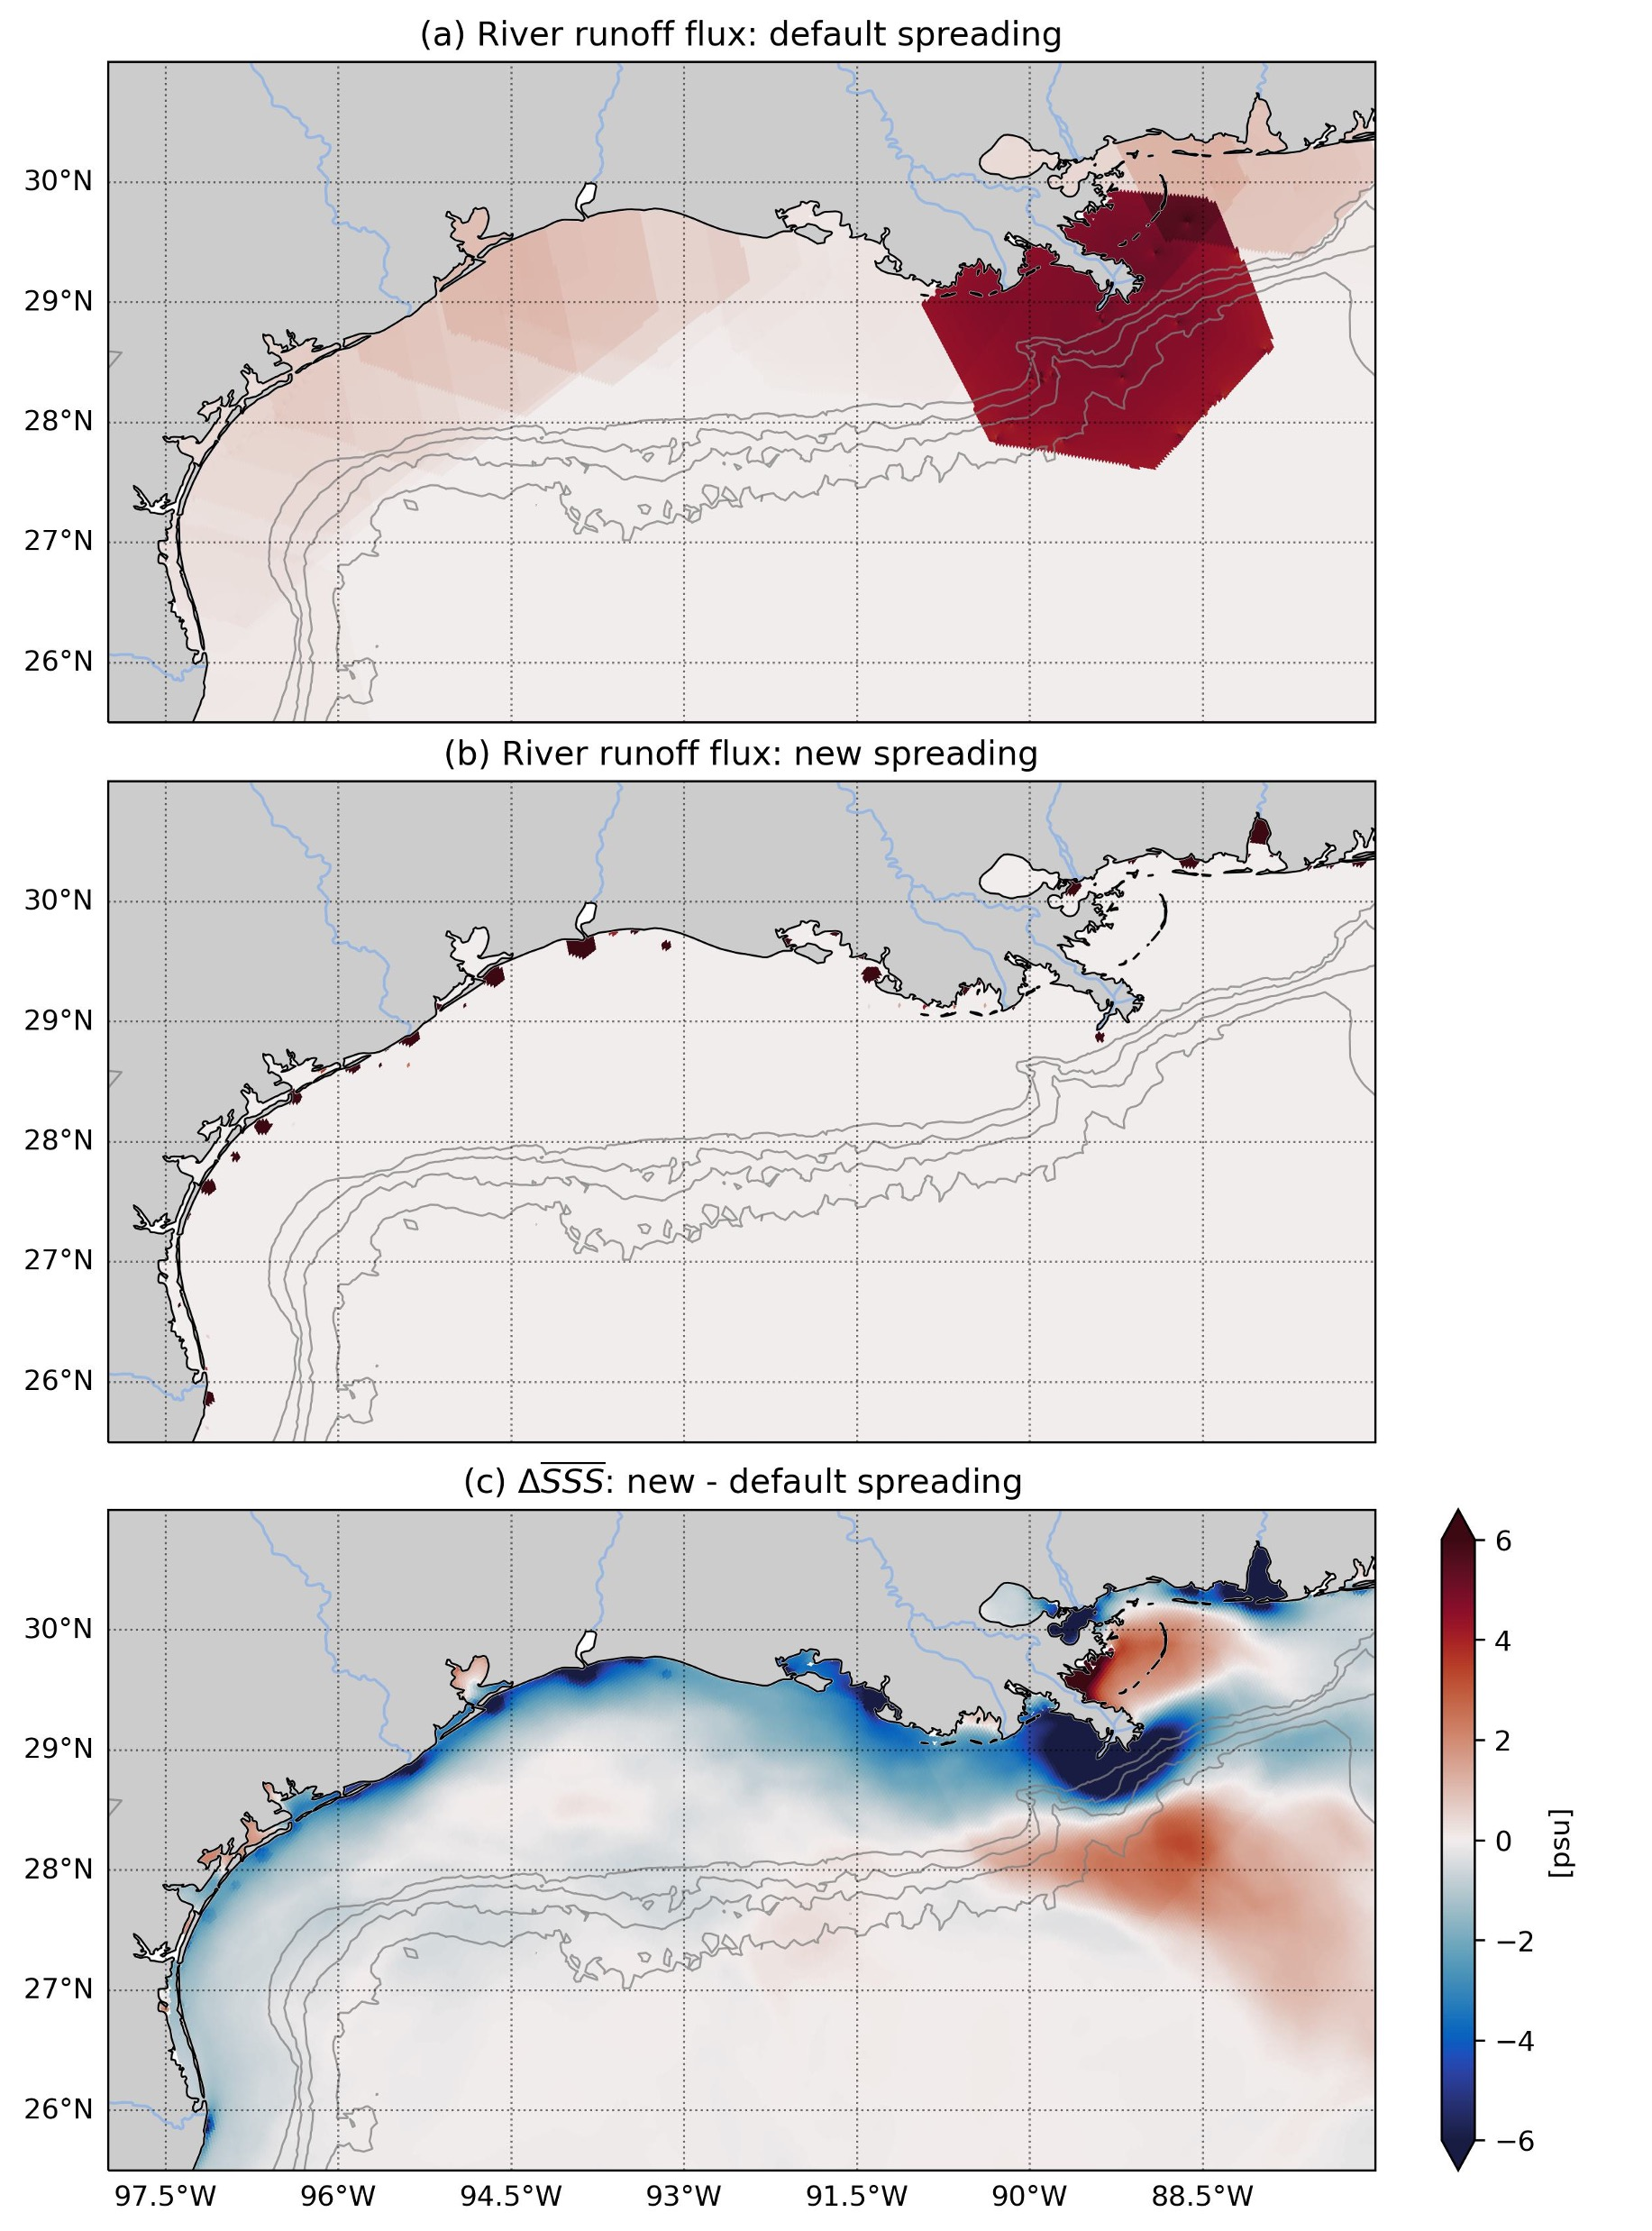
\includegraphics[width=0.95\textwidth]{figures/scgsr/spreading_comp.jpg}}
    \caption{Default river spreading implementation in E3SM v2 (a) and the new implementation developed for the GoM3 simulations (b). (c) Relative difference in the time-averaged sea surface salinity $\Delta \overline{SSS}$ between the new and default spreading for an eight month trial simulation during 1958.}
    \label{fig:spreading}
\end{figure}

The improvement of the new river spreading is shown in Fig. \ref{fig:spreading} (c) with the time-averaged change in sea surface salinity $\Delta SSS$ between the new and default spreading for an eight month trial simulation. The simulation was performed from Jan-Aug, 1958 with 128 vertical layers, 0.2 m layer thickness, and 4 m minimum water depth \footnote{This vertical mesh was later found to be unstable.}. The trial simulation results show the freshwater content over the shelf increases signficantly with the new spreading, with $\Delta \overline{SSS}$ values exceeding six psu near most of the major rivers. The default configuration spreads much of M. River water directly into deep water, which is physically unrealistic and distorted the structure of LC eddies as they are move onto the TXLA shelf (not shown). 

\begin{figure}[t]
\centerline{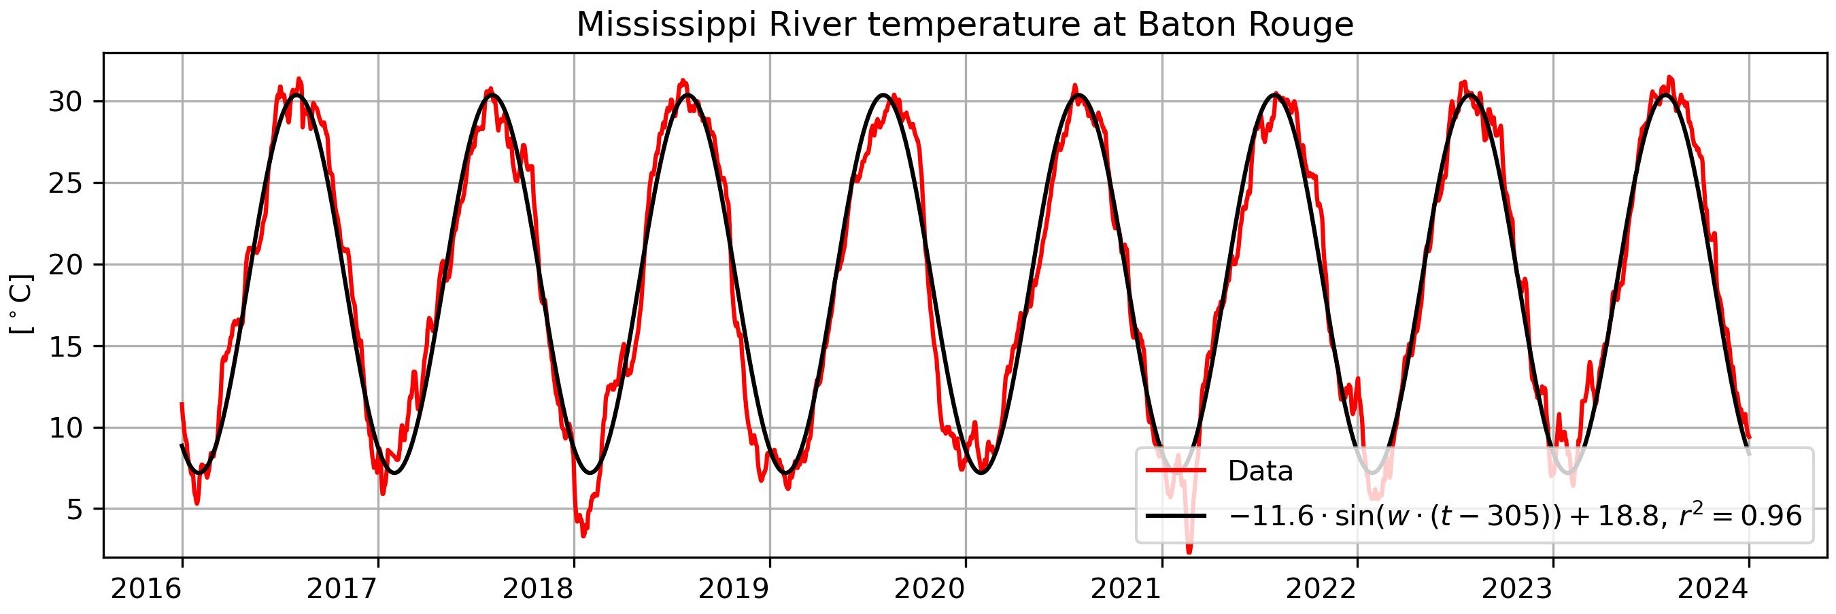
\includegraphics[width=\textwidth]{figures/scgsr/Miss_temp.jpg}}
    \caption{Time series of daily-averaged Mississippi river temperature and fitted sine wave.}
    \label{fig:miss_temp}
\end{figure}

We modified the temperature of the river runoff flux because of stability concerns that arose during vertical resolution experiments. E3SMv2 sets the river temperature equal to the ambient sea surface temperature at the river release location. Trial experiments (not shown) revealed that inflowing water at the spreading points of Southwest Pass was spuriously heated to unrealistic temperatures. To alleviate this issue, we set the inflowing runoff temperatures of all rivers in the GoM to a fitted sine function using eight years of USGS daily-averaged streamflow data at Baton Rouge (\url{https://waterdata.usgs.gov/monitoring-location/07374000}) that covers all years under JRA forcing (1958-present). While setting all inflowing river temperatures equal to the Mississippi is physically unrealistic, there is currently no simple way to apply this modification to only a subset of the rivers in E3SM, this solution guaranteed inflowing river water within the GoM was not spuriously heated, and the time scale of the effects of this solution propagating from regions of the global ocean where this is unrealistic is much longer than the simulations this study analyzes. 

The river temperature function ($\theta_{riv}$) is prescribed daily as
\begin{equation}
    \theta_{riv} = A \sin (\omega [t_{day}-t_{off}] ) + C, 
\end{equation}
where $A$ is the amplitude, $\omega$ is the angular frequency, $t_{day}$ is the model day of year, $t_{off}$ is phase offset, and $C$ is the vertical shift. Values for $A$, $\omega$, $t_{off}$, $C$, and goodness of fit ($r^2$) are shown in Fig. \ref{fig:miss_temp}. 

\subsection{GoM3 vertical meshes}
We developed 18 trial meshes and attempted to make these parameters comparable to the TXLA model. Due to stability issues, we designed a low (GoM3r1) and medium (GoM3r2) resolution vertical mesh with vertical grid parameters $h_{min} = (10,20)$ m, $z_{min} = (10,2)$ m, and $z_{lay} = (64,128)$, respectively. 

GoM3r1 was used for tuning experiments with $\nabla_0^4$ to get a sense of scale for the permitted submesocales in the outer GoM. GoM3r1 uses only three vertical layers where the bottom depth is 20 m and features roughly 10 vertical layers inshore of the 100 m depth. GoM3r2 uses 10 vertical layers at 20 m depth and roughly 50 vertical layers inshore of 100 m depth. While this resolution is insufficient to capture the upper structure of the M/A plume, the middle of the water column is better resolved than the TXLA model.

We determined the stability issues are related to model forcing because all trial meshes ran successfully in stand alone. For example, the highest resolution case used $z_{min} = 0.2$ m and $h_{min} = 1$ m and ran with no Rayleigh damping for one simulated year. Two general scenarios describe the stability issues. First, thin layers (e.g. $z_{min} = 0.2$ m) coupled with shallow bathymetry (e.g $h_{min}=3$ m) caused $z_{min}$ to become negative near the M/A rivers within the first few days of spinup. Second, thin vertical layers ($z_{min} = 0.2$) with unrealistic bathymetry ($h_{min}=10$ m) caused numerical instability at Southwest Pass to form within several months of simulated time, but $z_{min}$ remained positive. The exact cause of the stability issues is still under investigation. 

\subsection{Biharmonic horizontal mixing}
The representation of submesoscales in the GoM is sensitive to the biharmonic mixing coefficient $\nabla_0^4$ because it smooths energy at higher wavenumbers. For example, Fig. \ref{fig:del4} shows snapshots of surface normalized relative vorticity $\zeta f^{-1}$, where $\zeta = \partial_x v - \partial_y u$ and $f$ is the Coriolis parameter, for a simulation using $\nabla_0^4=2.0 \cdot 10^{11}$ [m$^4$s$^{-2}$]) and ($\nabla_0^4=3.33 \cdot 10^{11}$ [m$^4$s$^{-2}$]). The former is the target value selected from six tuning simulations (not shown), where smaller values of $\nabla_0^4$ were found to be unstable, and the latter is the default value used in lower resolution meshes. Higher $\nabla_0^4$ suppresses submesoscales within the GoM, which results in weaker surface fronts, secondary instabilities that form off the LC, and submesocale soup in the eastern GoM. 

\begin{figure} \centerline{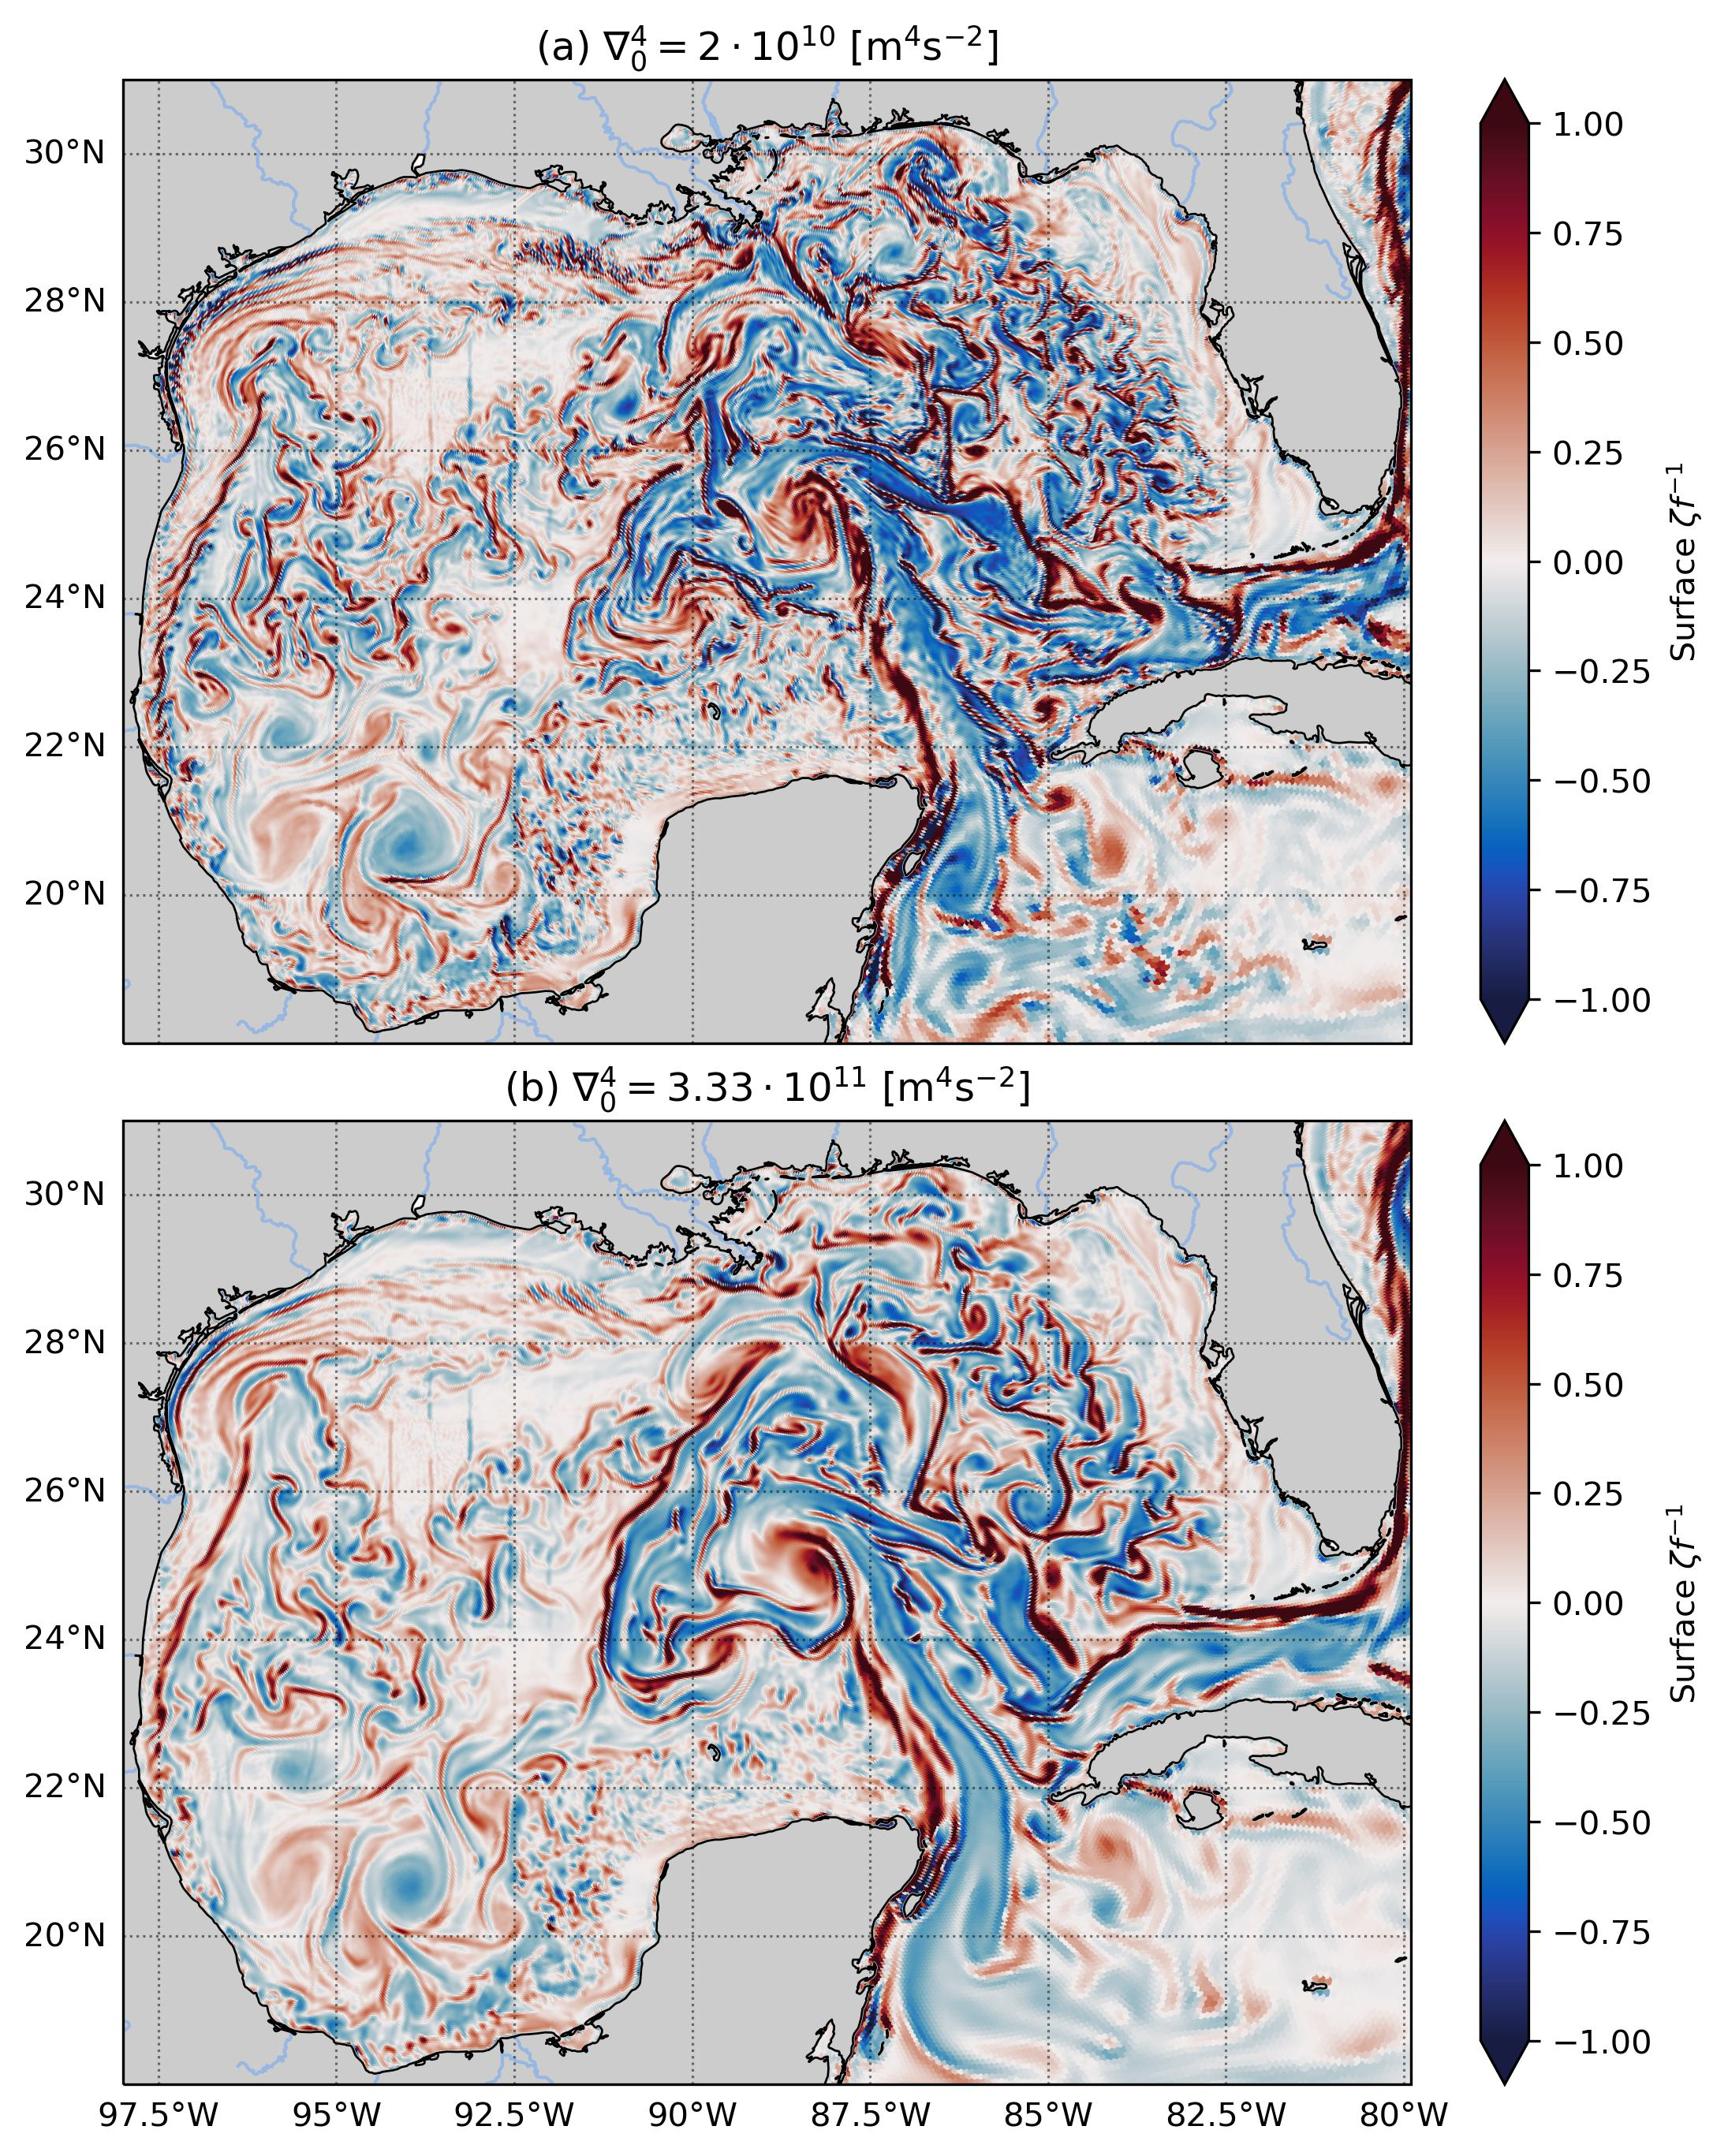
\includegraphics[width=\textwidth]{figures/scgsr/rvort_del4_comp.jpg}}
    \caption{Snapshots of GoM3r1 surface $\zeta f^{-1}$ for different $\nabla_0^4$ values on Feb 22, 1958.}
    \label{fig:del4}
\end{figure}

Periods of higher river discharge (fall and winter) required increases in $\nabla_0^4$ for both GoM3 meshes by over 50\% to maintain stability over the shelf. GoM3r2 required higher $\nabla_0^4$ values relative to GoM3r1 because sharper surface fronts are permitted at higher vertical resolution, especially within the M/A plume. We discuss the implications of this on the representation of surface fronts in the next section. 

\section{Results}
\subsection{Representation of surface vorticity}
Fig. \ref{fig:gom3_rvort_planview} shows snapshots of surface $\zeta f^{-1}$ for GoM3r1 and GoM3r2 during winter and summer. There is an abundance of submesoscale features including fronts, filaments, and eddies found in winter for both simulations. It is encouraging to see the development of secondary instabilities near LC eddies and submesoscale soup forming in the eastern GoM, consistent with previous studies \citep{Barkan_2017, bracco2019mesoscale, liu2021submesoscale}. There are less submesoscales than expected found during summer and frontal eddies seldom form inshore of 100 m depth over the TXLA shelf. Frontal eddies occasionally form over the continental slopes (Fig. \ref{fig:gom3_rvort_planview} c), however they are less organized than eddies found in the TXLA model and the vorticity is about half the magnitude \citep[compare to Fig. 2 of ][]{Schlichting23}. In addition, the submesoscales appear weaker in GoM3r2 despite the higher vertical resolution, which we suspect is due to the higher $\nabla_0^4$ required to maintain stability. 

\begin{figure}[t]
\centerline{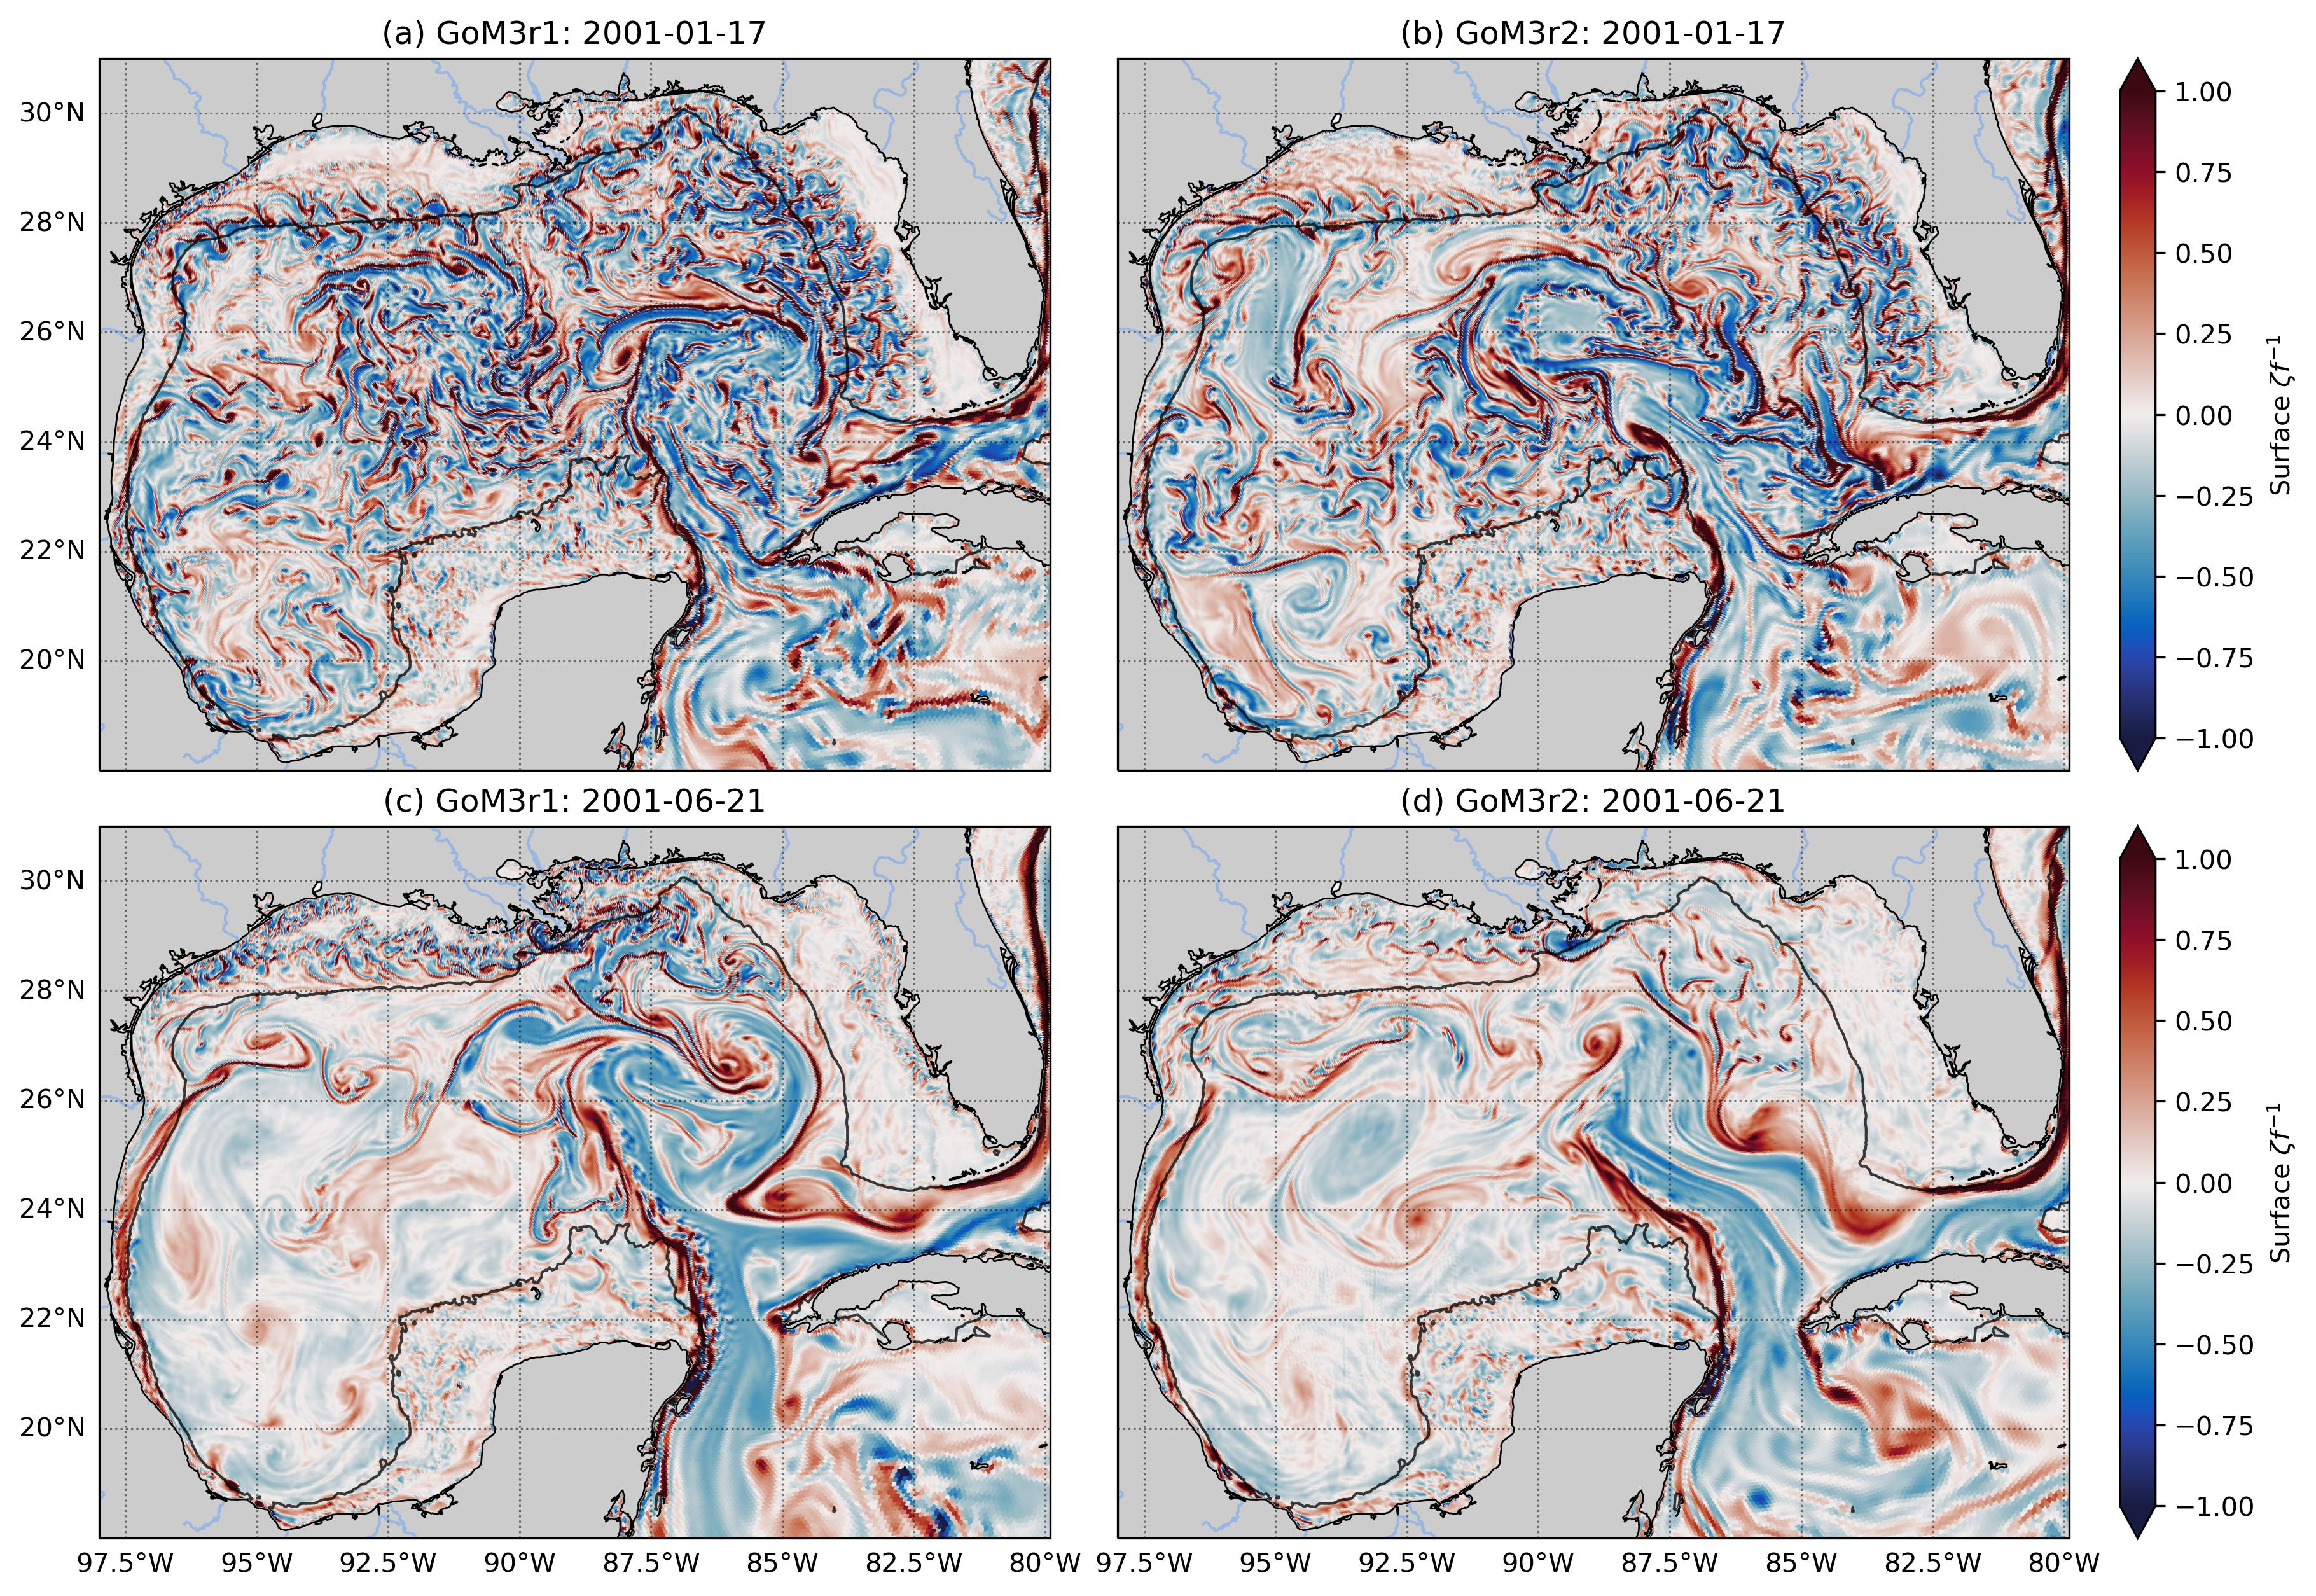
\includegraphics[width=\textwidth]{figures/scgsr/GoM3_rvort_comp2.jpg}}
    \caption{Snapshots of GoM3r1 (a) and GoM3r2 (b) surface $\zeta f^{-1}$ on Jan. 17, 2001. (c-d) same as (a-b), but on Jun. 26, 2001. The 100 m isobath is overlaid in black to show the shelf boundary.}
    \label{fig:gom3_rvort_planview}
\end{figure}

We examine the statistical representation of submesoscales in the GoM3 simulations using probability density functions (PDFs) of surface $\zeta f^{-1}$ for the entire GoM and TXLA shelf (Fig. \ref{fig:pdfs_gom}). The TXLA shelf is subsetted to the location of the child grid shown in \cite{Schlichting23} because frontal eddies are commonly found in this region. The prevalence of submesoscales are often indicated by elongated positive tails (cyclonic vorticity) in the PDF and a peak negatively offset from zero (anticyclonic vorticity) \citep{McWilliams_2016, Shcherbina_2013, taylor2023submesoscale}. Based on previous TXLA model results \citep{Schlichting23}, we anticipate a peak offset that is more pronounced over the shelf because the anticyclonic cores of frontal eddies saturate the shelf. 

\begin{figure}[t]
\centerline{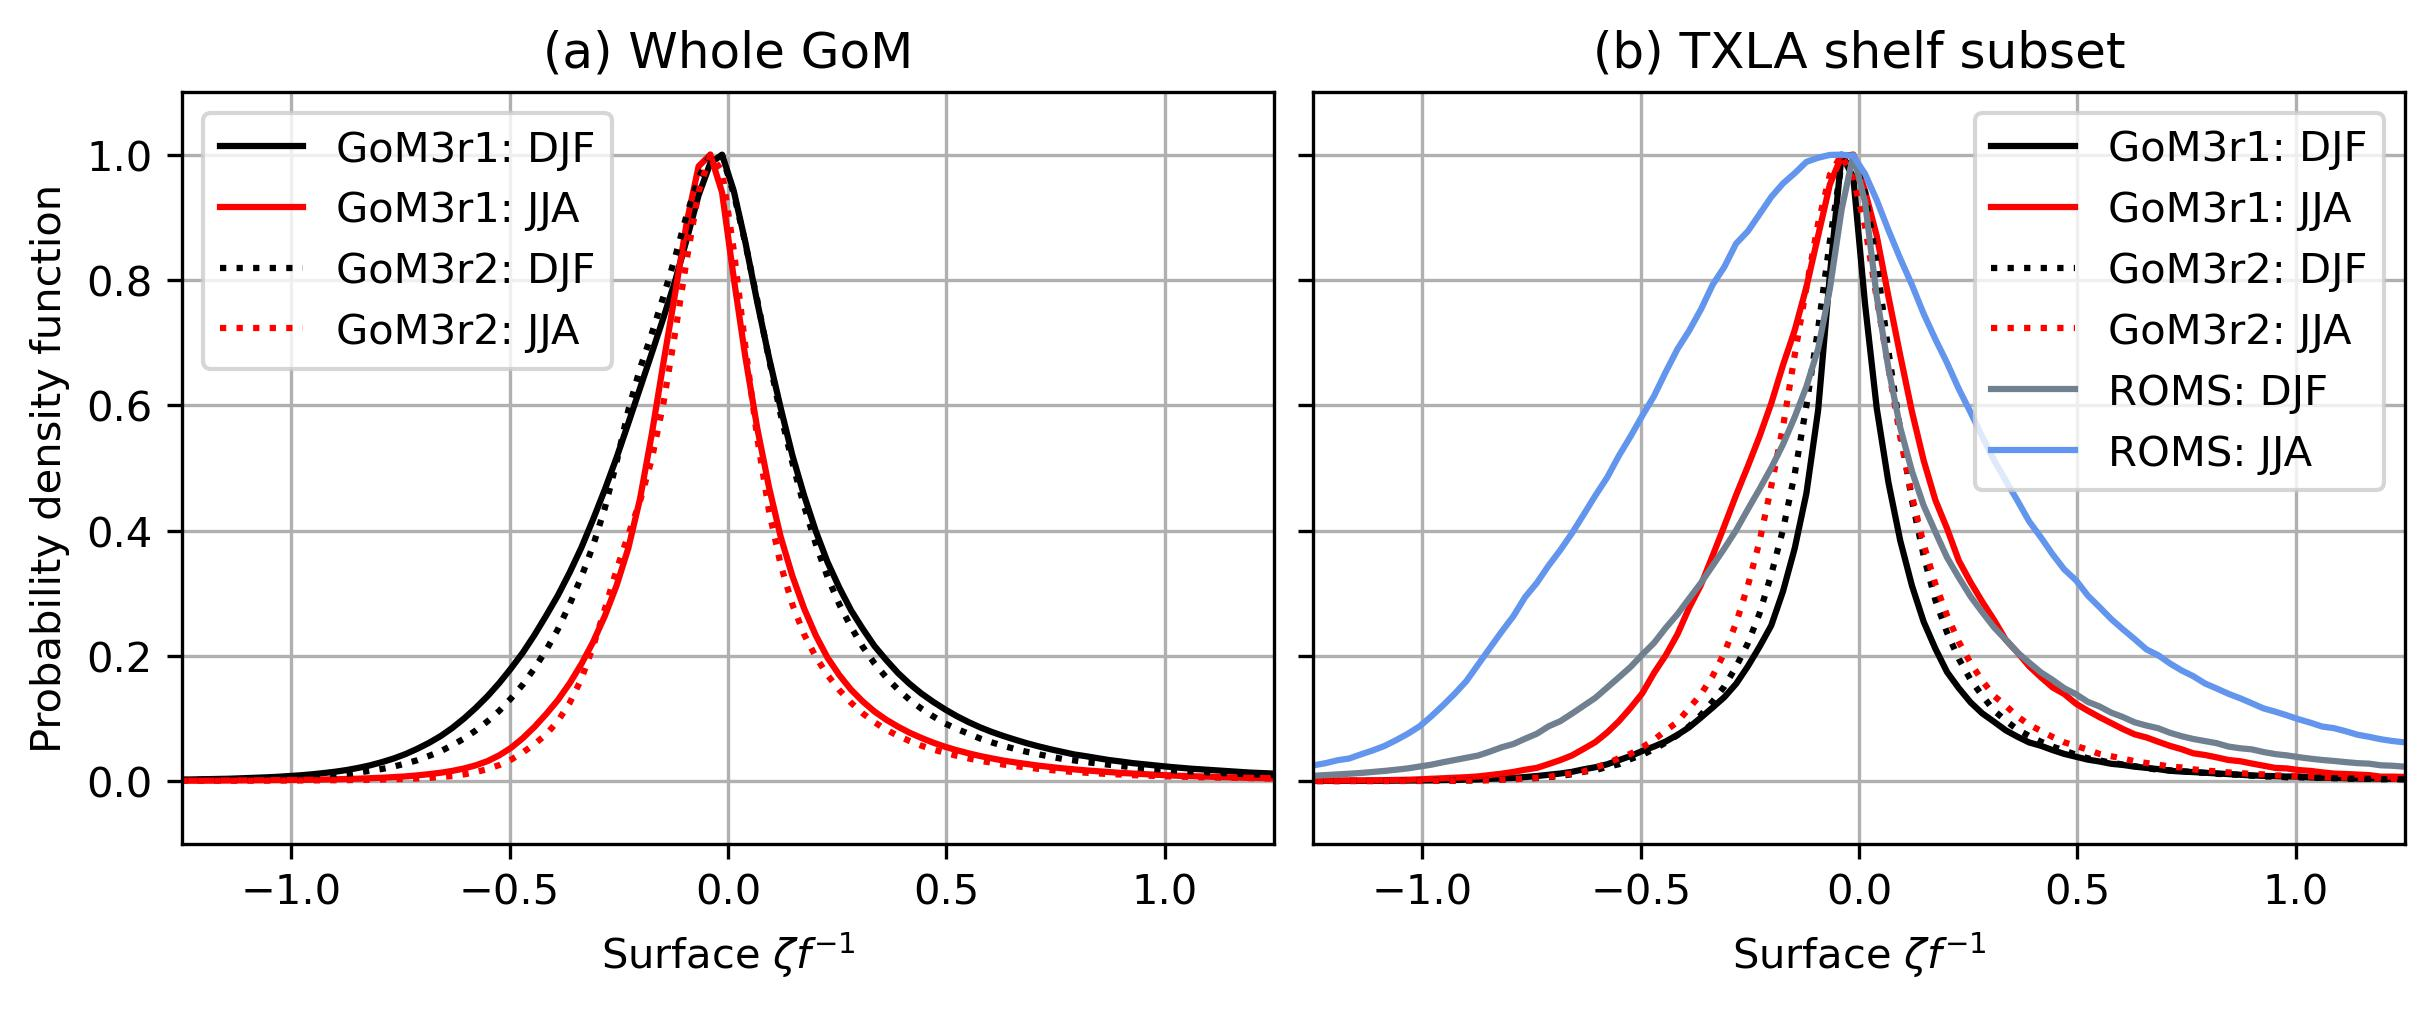
\includegraphics[width=\textwidth]{figures/scgsr/mpaso_roms_vortpdf.jpg}}
    \caption{Winter and summer probability density functions of surface $\zeta f^{-1}$ for the entire GoM (a) and TXLA inner shelf (b). The TXLA ROMS model is included in (b) for comparison.}
    \label{fig:pdfs_gom}
\end{figure}

For the whole GoM (Fig. \ref{fig:pdfs_gom} a), the GoM3 simulations feature a peak slightly offset from zero and tails that are just starting to elongate. For GoM3r1 during winter, less than one in every thousand cells (i.e. $PDF<10^{-3}$) falls within $\zeta f^{-1} = [-1.65,2.0]$. There are instances of stronger vorticity in winter than summer, indicating submesoscales are more prevalant in winter, which is consistent with Fig. \ref{fig:gom3_rvort_planview}. PDFs of GoM3r1 and GoM3r2 are very similar, with slightly stronger values found in GoM3r1.

For the TXLA shelf, the TXLA model produces a positively skewed PDF in summer with a peak further offset from zero than any GoM3 simulation due to a rich baroclinic eddy field (not shown). In winter, fewer submesoscales are found, resulting in a more symmetric PDF. However, the TXLA model during winter features stronger vorticity than both GoM3 simulations. This is due to two reasons, the mean horizontal resolution of the TXLA model is about 1.5 km in the region where the PDFs are computed, and the GoM3 simulations never develop an eddy field. Another interesting result is that GoM3r1 features stronger vorticity over the shelf relative to GoM3r2 despite the very low vertical resolution. Thus, until we solve the stability issues, it is unclear to what extent MPAS-O can represent submesoscales over the TXLA shelf. 

\subsection{Structure of the M/A river plume}
Figs. \ref{fig:mpaso_sss}-\ref{fig:ROMS_sss} display seasonally averaged sea surface salinity (SSS) for winter and summer for the GoM simulations and TXLA model, respectively. Note that we consider the TXLA model to be the reference because the salinity field has been validated twice and the errors are unbiased \citep{Kobashi_2020, Zhang_2012_numerical}. The 33 psu isohaline is indicated by the black line, which marks the edge of the M/A River plume \citep{hetland2012integrated, thyng2018seasonal}. In addition, this comparison is intended for qualitative purposes only because the TXLA model is forced with ERA interim datasets, not JRA.

\begin{figure}
\centerline{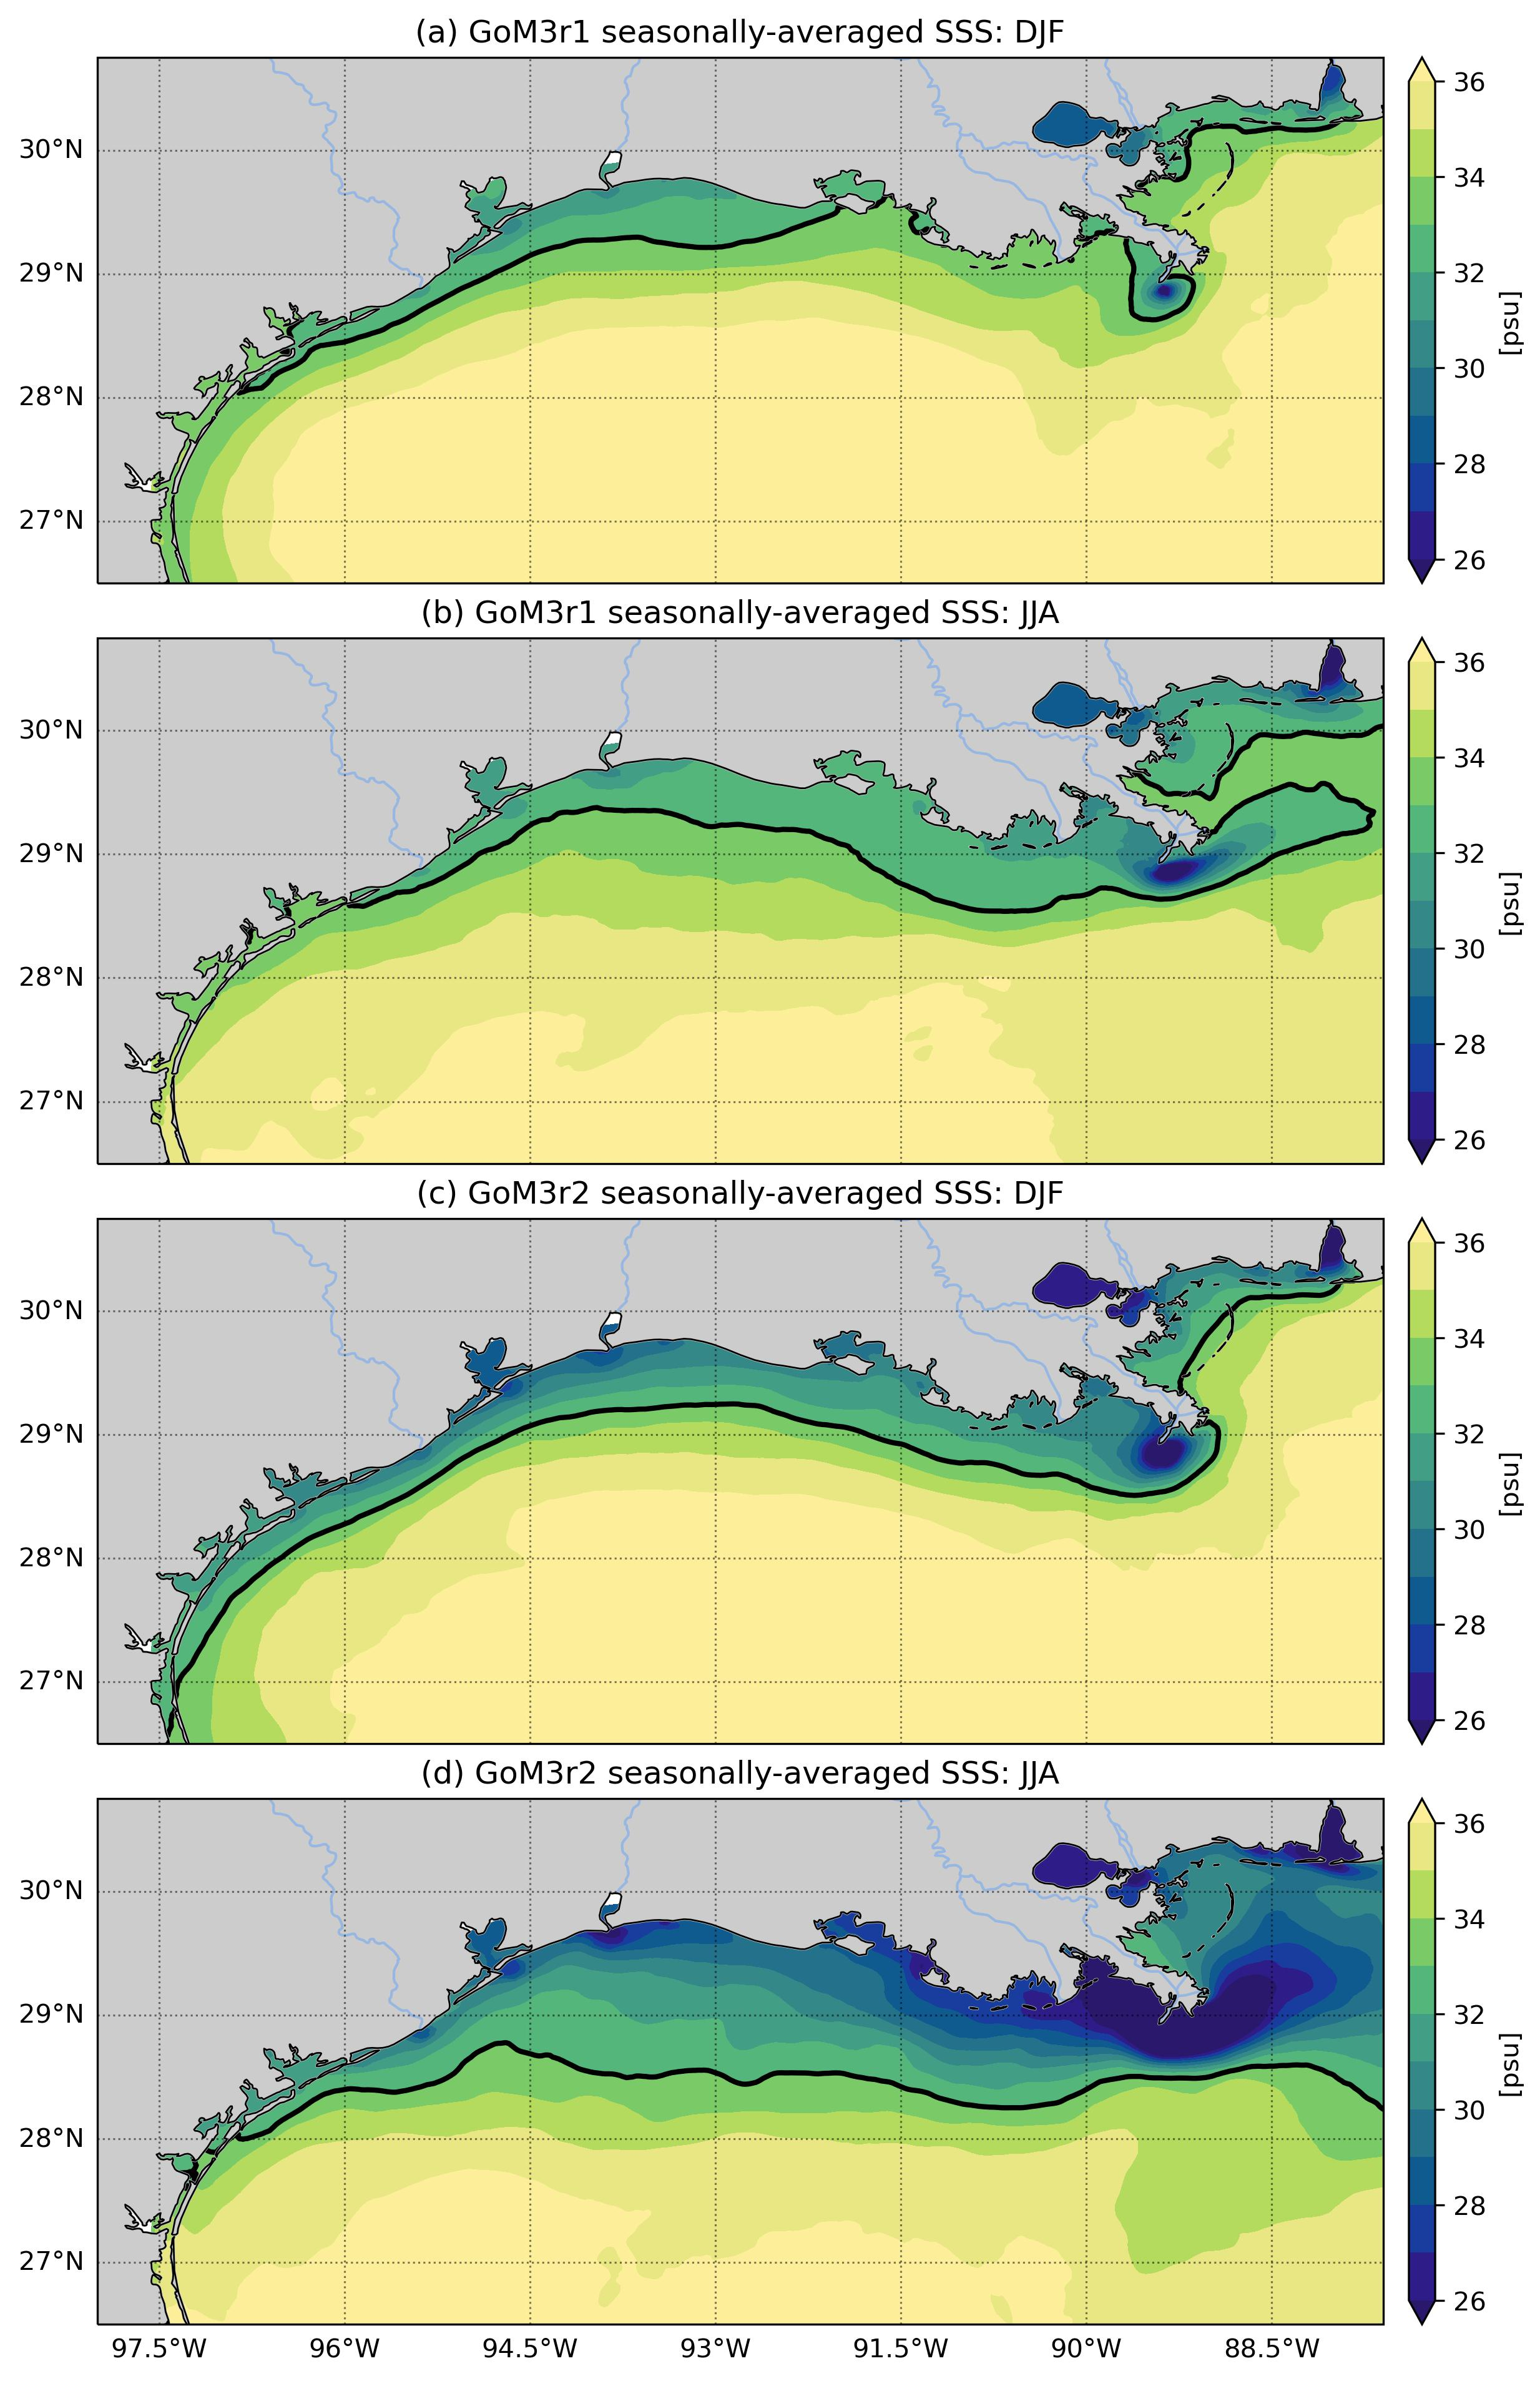
\includegraphics[width=0.82\textwidth]{figures/scgsr/mpaso_sss_mean.jpg}}
    \caption{Snapshots of the GoM3r1 seasonally averaged SSS for winter (a) and summer (b). (c-d) are the same as (a-b), but for GoM3r2. The black line marks the 33 psu isohaline.}
    \label{fig:mpaso_sss}
\end{figure}

\begin{figure}[t]
\centerline{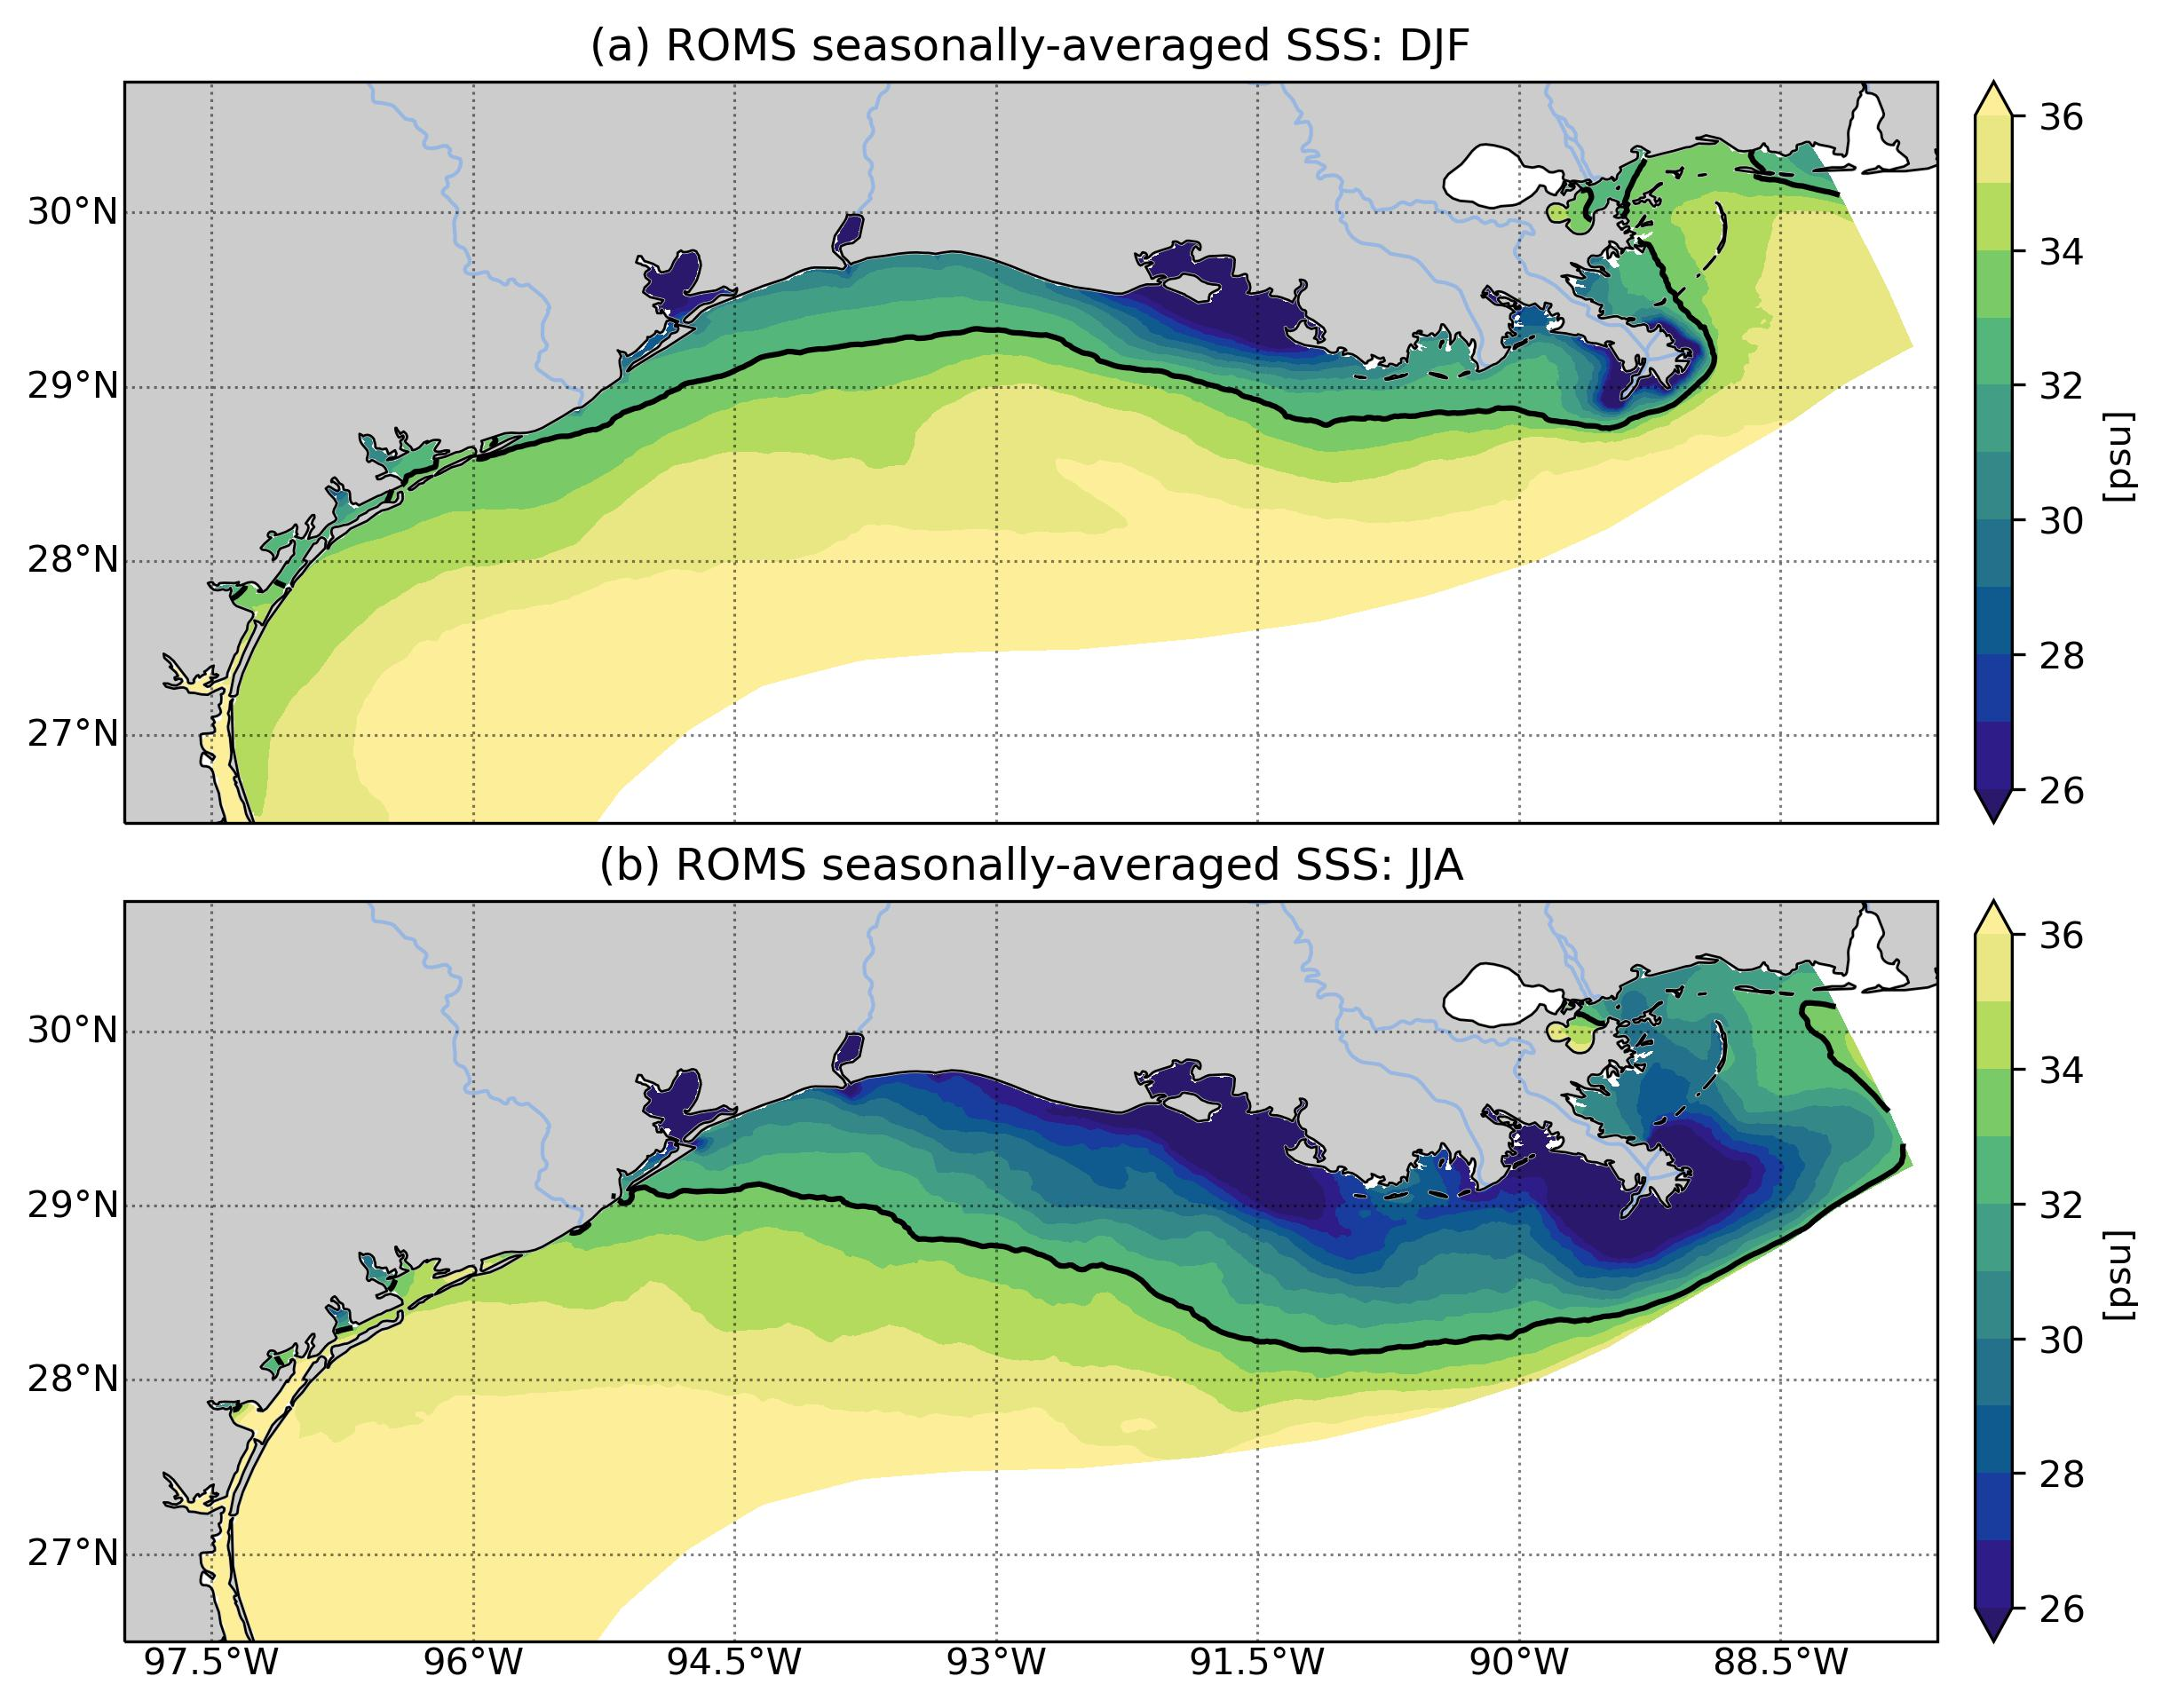
\includegraphics[width=0.82\textwidth]{figures/scgsr/txla_sss_mean.jpg}}
    \caption{Same as Fig. \ref{fig:ROMS_sss}, but for the TXLA model.}
    \label{fig:ROMS_sss}
\end{figure}

Despite the more "submesoscale" nature of GoM3r1's vorticity statistics, the river plume is poorly represented for both seasons and much of the shelf is too salty. This is an expected result given the low vertical resolution and the minimum water depth of 20 m. GoM3r2 produces a plume that is more qualitatively consistent with the TXLA model for both seasons and has a much more pronounced plume during summer relative to GoM3r1 despite not having an eddy field. However, we note that GoM3r2 is too salty in Atchafalaya Bay, along the other passes of Bird's foot, and near Port Arthur and Galveston Bay. In addition, GoM3r2 is too fresh over the western half of the TX shelf. 

We suspect the issues pertaining to Atchafalaya Bay and Bird's Foot are due to the lack of hydraulic control structure within JRA forcing and the river spreading still being too large, although this requires further investigation. That is, we suspect JRA forcing does account for United States Army Corps of Engineers modulation of Atchafalaya river fluxes. On the other hand, the TXLA model uses USGS streamflow data directly at the mouth of Atchafalaya Bay. Regarding the saltiness along the other passes of Bird's foot, this is because E3SM lacks a means to proportion the river fluxes through the other passes (as mentioned previously). Finally, we suspect the surplus of fresh water on the western TX shelf is because the river spreading is still too high, even with the newer spreading capabilities.

\section{Discussion and conclusions}
\subsection{Model strengths and limitations}
A current strength of the approach taken here is the GoM3 meshes have 345 thousand horizontal cells, which is low compared to other high resolution MPAS-O meshes \citep{caldwell2019doe, hoch2020mpas} and roughly three times as many horizontal cells as the TXLA model. This allows the quicker tuning of key subgrid scale parameterizations such as harmonic and biharmonic lateral mixing, GM, and Redi coefficients. However, this likely comes at the cost of being able to produce high-fidelity climate simulations. One solution is to regenerate the mesh and increase resolution outside the region of interest once the parameterizations have been tuned. Another strength is the representation of submesoscales within the broader GoM despite the coarse vertical resolution. The permission of seasonal variability is encouraging and we expect this to improve if higher horizontal resolution is used. 

The two biggest limitations preventing MPAS-O from being capable of producing high fidelity simulations of the TXLA shelf are vertical mesh stability issues and the river spreading. Notwithstanding stability issues, model fidelity is still constrained by river spreading. Although a river's spreading distance is set to be proportional to the inflowing flux, any spreading is physically unrealistic and will likely produce a fresh bias in most coastal regions. Even when individual river spreading is modified to be as small as stability constraints allow, it may be difficult or impossible to account for hydraulic control structures within the broader E3SM framework or when model forcing is run with reanalysis data. A potential option for future simulations is to incorporate rivers as point sources, as often done in many regional models. However, it is unclear if this could be done for stability reasons.

We note two experimental additions to the MPAS-O code that were not tested here but may be useful to future studies. One is the addition of a hybrid $\sigma-z$ vertical coordinate, which features a terrain following ($\sigma$) coordinate in the coastal ocean (the inner continental shelves/slopes) and transition to $z^*$ coordinates over the open open. The other addition is the inclusion of the Generic Length Scale (GLS) vertical mixing scheme configured as part of the General Ocean Turbulence Model \citep{burchard1999gotm, Warner_2005}, which has been shown to perform well in coastal models. 

In addition, we list several aspects of model configuration in approximate order of priority required to produce high fidelity simulations of coastal submesoscales that may be useful for future projects: 1) horizontal resolution, 2) vertical resolution, including an appropriate vertical coordinate for the region of interest, 3) realistic forcing, and 4) appropriately tuned subgrid-scale parameterizations. It should be noted that these components are inextricably linked and their order may differ depending on the project objectives. 

The horizontal resolution is the dominant factor affecting the resolved dynamics because it determines the Rossby number. High vertical resolution is necessary when the focus in on boundary- or mixed layer processes, and the vertical transport of material across- and within these layers. A heuristic argument can be made for the necessity of high quality forcing. The model will be as realistic as the forcing given to it. And finally, parameter tuning must be done on a per-mesh basis. Poorly tuned $\nabla_0^4$ can suppress submesoscales even if all other aspects of model configuration are optimized.

\subsection{Regional refinement compared to model nesting}
An alternative to the approach taken here is to one-way nest a regional model like ROMS into MPAS-O, which is currently being undertaken by the SEAHOR\c{C}E project (\url{https://github.com/seahorce-scidac}). An advantage of this approach is that ROMS is a mature regional ocean model specifically designed for simulations of estuarine and coastal flows with well understood strengths and limitations. Additionally, decades of work have gone into tuning and calibrating ROMS for the GoM region, while E3SM has historically had a more global focus to date. ROMS also features several options for tracer advection and vertical turbulence closure schemes in addition to KPP that can be experimented with to improve model performance. Particularly relevant for this work is that tracers can be treated as point sources such that anthropogenic hydraulic controls at discharge points can be easily accounted for. ROMS is also not prone to stability issues when run at high vertical resolution.

Besides creating robust code infrastructure to do the nesting, a major expected limitation of this approach is the computational cost. Model nesting has a additional computational overhead because information must be calculated at the lateral boundaries of each timestep and the inter-grid communication performance is dependent on a machine's hardware. The child grid will also require a finer timestep, which will slow computational speed. There is a similar issue in regionally refined MPAS-O meshes because the same timestep is applied to all cells. A possible remedy is to expand the local time stepping scheme \citep{lilly2023storm} to baroclinic applications. For the current MPAS-O code base, regional refinement appears to be a more practical option for open ocean regions (e.g. the Gulf stream) that are not signficantly influenced by river forcing and do not require $\mathcal{O}$(0.1 m) vertical resolution. These two approaches can be better compared when performance tests for nesting ROMS into MPAS-O are available. 

\section{Conclusions and future work}
We presented the development of an unprecedented 2.8 km resolution regionally refined mesh in the Gulf of Mexico (GoM) using the Model for Prediction Across Scales-Ocean (MPAS-O). The mesh, named GoM3, is intended to assess the representation of coastal submesoscale processes over the Texas-Louisiana (TXLA) shelf and the broader GoM. Our case study approach is motivated by the pronounced submesoscale eddy field that develops over the Mississippi and Atchafalaya (M/A) River plume over the TXLA shelf during summer and the strong seasonal variability of submesoscales within the broader GoM. The lateral density gradients of both regions are strongly modulated by regional rivers and the larger-scale mesoscale circulation, so we think this represents a challenging test to study submesoscales with regionally refined meshes. Our benchmark for comparison is a validated implementation of the Regional Ocean Modeling System (ROMS), the TXLA model, which covers the TXLA shelf and outer continental slopes. 

The horizontal mesh is gradually relaxed to 60 km in the broader Atlantic and Southern Oceans and to 100 km in the Pacific and Indian Oceans. MPAS-O is coupled with MPAS-Sea Ice to produce a realistic Atlantic Meridional Overturning Circulation such that a realistic loop current is produced. The simulations are forced with Japanese 55 year reanalysis datasets (JRA). Preliminary results suggest this configuration is not suitable for long-term climate simulations due to the low resolution regions, but further testing is required. We described improvements made to how river forcing is applied in the model, including the spreading and inflowing temperatures. We also found the representation of submesoscales to be sensitive to the amount of prescribed biharmonic lateral mixing. 

We ran two coupled numerical simulations using a low (GoM3r1) and medium (GoM3r2) vertical resolution mesh from 2000-2001 following a two year spinup. We were unable to produce a vertical mesh with comparable resolution and minimum bathymetry to the TXLA model due to stability issues. Both simulations do not produce a submesoscale eddy field over the TXLA shelf. However, they both permit submesoscales in the broader GoM and begin to produce seasonal variability found in previous studies \citep{Barkan_2017, liu2021submesoscale}. GoM3r1 produces a low quality representation of the M/A river plume due to the coarse vertical resolution, but has slightly more submesoscale features in the broader GoM than GoM3r2. This is because GoM3r2 required twice the biharmonic mixing as GoM3r1 to maintain stability. Despite the lack of submesoscale eddies, seasonal averages of sea surface salinity showed GoM3r2 produced a higher quality M/A river plume structure that starts to resemble the TXLA model. Major issues are over a salty bias near Atchafalaya Bay and a fresh bias off the southern TX coast, which we suspect is related to issues with river spreading and a lack of hydraulic control structure within JRA forcing. We plan to take several actions in future work described below to improve MPAS-O's representation of submesoscales over the TXLA shelf.

Assuming the vertical stability issues can be fixed, our next GoM3 simulation will target a 0.5 m minimum layer thickness and five m minimum water depth so it is comparable with the TXLA model. We will reduce the Atchafalaya River spreading to be similar to the Mississippi and examine where JRA forcing accounts for the hydraulic control structure over the M/A rivers. We also plan to generate a new horizontal mesh with 1.5 km resolution so it is comparable with the TXLA model in the region of interest. This will also allow us to compare model results in the broader GoM directly with previous studies that have already produced simulations at this resolution \citep{Barkan_2017, bracco2019mesoscale, liu2021submesoscale}. Ideally, we will run the TXLA model with JRA forcing so it can be compared directly with MPAS-O, which is especially important if JRA forcing lacks the hydraulic control between the M/A rivers. 

Regarding analysis, we will implement an idealized passive tracer that is intended to serve as a proxy for freshwater content over the shelf. We will compare monthly-averaged seasonal sections of the active and passive tracers between models, which can allow us to infer information abut the performance of KPP in coastal settings. We plan to add the approach by \cite{Klingbeil_2014} to quantify numerical mixing, the spurious mixing generated by the discretization of advection, to the MPAS-O code. Little work has been done in quantifying numerical mixing in MPAS-O simulations besides the approach by \cite{winters1995available}, which is restricted to reference potential energy integrated over entire control volumes.

